\documentclass[10pt,letterpaper]{article}

\usepackage[margin=0.75in, headheight=15pt]{geometry}
\usepackage{amsmath,amssymb}
\usepackage{booktabs}
\usepackage{longtable}
\usepackage{array}
\usepackage{tabularx}
\usepackage{xcolor}
\usepackage{graphicx}
\usepackage{tikz}
\usetikzlibrary{arrows.meta,positioning,shapes.geometric,fit,backgrounds,calc}
\usepackage{pgfplots}
\pgfplotsset{compat=1.18}
\usepackage{microtype}
\usepackage{xurl}
\usepackage{hyperref}
\usepackage{enumitem}
\usepackage{fancyhdr}
\usepackage{multicol}
\usepackage{placeins}
\usepackage{titlesec}
\setlength{\emergencystretch}{2.2em}
\setlength{\parindent}{0pt}
\setlength{\parskip}{4.5pt}

% ============================================================================
% COLOR PALETTE (MATCHING LIVE PLANARIA v2.4 STUDIO THEME)
% ============================================================================
\definecolor{plnBg}{HTML}{0B1320}
\definecolor{plnSlate}{HTML}{1E293B}
\definecolor{plnMuted}{HTML}{475569}
\definecolor{plnBorder}{HTML}{CBD5E1}
\definecolor{plnSoft}{HTML}{F8FAFC}
\definecolor{plnEmerald}{HTML}{059669}
\definecolor{plnEmeraldBg}{HTML}{ECFDF5}
\definecolor{plnCyan}{HTML}{0284C7}
\definecolor{plnCyanBg}{HTML}{F0F9FF}
\definecolor{plnGold}{HTML}{D97706}
\definecolor{plnGoldBg}{HTML}{FFFBEB}
\definecolor{plnCrimson}{HTML}{DC2626}
\definecolor{plnCrimsonBg}{HTML}{FEF2F2}
\definecolor{plnViolet}{HTML}{7C3AED}
\definecolor{plnVioletBg}{HTML}{F5F3FF}
\definecolor{plnMagenta}{HTML}{C026D3}

\hypersetup{
  colorlinks=true,
  plainpages=false,
  linkcolor=plnCyan,
  citecolor=plnEmerald,
  urlcolor=plnCyan,
  pdftitle={PLANARIA v2.4 Complete GUI Operator Manual, Architecture Atlas and Visual Field Guide},
  pdfauthor={Alexander Stephen Donahue (Independent Researcher, 0thernes project, ORCID 0009-0006-8168-9648)},
  pdfsubject={Complete illustrated guide to every control, HUD readout, quantum/temporal model, surgical vivisection tool, Proof Blueprint, CLI command, and verification artifact in PLANARIA v2.4.0}
}

% Styled headings
\titleformat{\section}
  {\Large\bfseries\sffamily\color{plnBg}}
  {\colorbox{plnCyan}{\color{white}\normalsize\bfseries\;\thesection\;}}
  {0.6em}{}[\vspace{2pt}{\color{plnCyan}\titlerule[1.2pt]}]

\titleformat{\subsection}
  {\large\bfseries\sffamily\color{plnSlate}}
  {\color{plnEmerald}\thesubsection}
  {0.55em}{}

\titleformat{\subsubsection}
  {\normalsize\bfseries\sffamily\color{plnCyan}}
  {\thesubsubsection}
  {0.5em}{}

% Header / Footer
\pagestyle{fancy}
\fancyhf{}
\fancyhead[L]{\footnotesize\sffamily\color{plnMuted}PLANARIA v2.4.0 --- COMPLETE GUI OPERATOR MANUAL \& VISUAL FIELD GUIDE}
\fancyhead[R]{\footnotesize\sffamily\color{plnMuted}DONAHUE (0THERNES)}
\fancyfoot[L]{\footnotesize\sffamily\color{plnMuted}\nolinkurl{https://0thernes.github.io/planaria/}}
\fancyfoot[R]{\footnotesize\sffamily\color{plnSlate}\textbf{Page \thepage}}
\renewcommand{\headrulewidth}{0.4pt}
\renewcommand{\footrulewidth}{0.3pt}

% Reusable callout boxes built cleanly with TikZ (zero external box package dependencies)
\newcommand{\calloutbox}[4]{%
  \par\medskip\noindent
  \begin{tikzpicture}
    \node[
      draw=#1,
      fill=#2,
      line width=0.9pt,
      rounded corners=3pt,
      inner sep=8pt,
      text width=\dimexpr\textwidth-18pt\relax,
      align=left
    ] (box) {%
      {\sffamily\bfseries\color{#1}#3}\par\smallskip
      {\small #4}
    };
  \end{tikzpicture}\par\medskip
}

% Compact keyboard badge
\newcommand{\kbd}[1]{%
  \tikz[baseline=(char.base)]{%
    \node[draw=plnSlate!60, fill=plnSoft, rounded corners=2pt, inner xsep=3.2pt, inner ysep=1.2pt, font=\scriptsize\ttfamily\bfseries] (char) {#1};%
  }%
}

% Compact pill badge
\newcommand{\pill}[2]{%
  \tikz[baseline=(char.base)]{%
    \node[draw=#1, fill=#1!12, text=#1, rounded corners=2pt, inner xsep=3.5pt, inner ysep=1.2pt, font=\scriptsize\sffamily\bfseries] (char) {#2};%
  }%
}

\newcolumntype{L}[1]{>{\raggedright\arraybackslash}p{#1}}
\newcolumntype{Y}{>{\raggedright\arraybackslash}X}

\begin{document}

% ============================================================================
% COVER PAGE
% ============================================================================
\begin{titlepage}
\pagenumbering{Alph}
\thispagestyle{empty}
\begin{tikzpicture}[remember picture, overlay]
  \fill[plnBg] (current page.north west) rectangle ([yshift=-8.75cm]current page.north east);
  \fill[plnEmerald] ([yshift=-8.75cm]current page.north west) rectangle ([yshift=-8.93cm]current page.north east);
  \fill[plnCyan] ([yshift=-8.93cm]current page.north west) rectangle ([yshift=-9.05cm]current page.north east);
\end{tikzpicture}

\vspace*{0.35cm}
{\sffamily\color{plnEmerald}\bfseries\small 0THERNES RESEARCH PROJECT $\;\cdot\;$ ILLUSTRATED TECHNICAL REFERENCE \& FIELD MANUAL $\;\cdot\;$ RELEASE v2.4.0}

\vspace{0.5cm}
{\sffamily\color{white}\Huge\bfseries PLANARIA v2.4}\\[0.25cm]
{\sffamily\color{white!88!cyan}\Large\bfseries Complete GUI Operator's Manual, Visual Field Guide,\\
Architecture Atlas, Step-by-Step Lab Handbook \& Glossary}

\vspace{0.5cm}
{\sffamily\color{white!82!gray}\normalsize
Every screen zone, button, slider, HUD readout, quantum observable, temporal engine mechanic, 1/1 procedural generator table, 192-cell binary tissue map, vascular anastomosis route, Plang compiler panel, surgical vivisection control, 48~kHz AudioWorklet DSP stage, 85-theorem Proof Blueprint inspector, and CLI command --- explained completely with diagrams, charts, formulas, and hands-on lab protocols.}

\vspace{1.25cm}

% At-a-Glance Metadata Card
\begin{tikzpicture}
  \node[draw=plnBorder, fill=plnSoft, rounded corners=4pt, inner sep=10pt, text width=\dimexpr\textwidth-22pt\relax] {
    \begin{tabularx}{\linewidth}{@{} L{3.6cm} Y @{}}
      \textbf{\sffamily Author} & Alexander Stephen Donahue --- Independent Researcher (\href{https://0thernes.art}{0thernes project}, Spokane, WA, USA) \\
      \textbf{\sffamily ORCID / Contact} & \href{https://orcid.org/0009-0006-8168-9648}{\texttt{0009-0006-8168-9648}} $\cdot$ \href{mailto:0_0@0thernes.art}{\texttt{0\_0@0thernes.art}} \\
      \textbf{\sffamily Live Interactive GUI} & \href{https://0thernes.github.io/planaria/}{\nolinkurl{https://0thernes.github.io/planaria/}} \\
      \textbf{\sffamily Interactive Blueprint} & \href{https://0thernes.github.io/planaria/blueprint/}{\nolinkurl{https://0thernes.github.io/planaria/blueprint/}} (85 Lean~4.35.0 theorems) \\
      \textbf{\sffamily Source \& Release} & \href{https://github.com/0thernes/planaria}{\nolinkurl{https://github.com/0thernes/planaria}} $\cdot$ Release \texttt{v2.4.0} \\
      \textbf{\sffamily Research Archive ID} & \texttt{0TH-BUILD-002} in \href{https://github.com/0thernes/0thernes-research-archive}{\nolinkurl{0thernes-research-archive}} \\
      \textbf{\sffamily Edition / Date} & Complete Illustrated Manual v2.4.0 $\cdot$ November 26, 2026 \\
      \textbf{\sffamily License} & Cosmogonic License --- Non-Commercial Research \& Play (audit tooling CC~BY~4.0) \\
    \end{tabularx}
  };
\end{tikzpicture}

\vspace{0.55cm}

% Scorecard Strip
\noindent\textbf{\sffamily\color{plnSlate}VERIFIED SYSTEM SCORECARD (PLANARIA v2.4.0)}
\vspace{4pt}

\begin{center}
\footnotesize
\begin{tabularx}{\textwidth}{@{} >{\centering\arraybackslash}X >{\centering\arraybackslash}X >{\centering\arraybackslash}X >{\centering\arraybackslash}X @{}}
\toprule
\textbf{\color{plnEmerald}85 / 85 Theorems} & \textbf{\color{plnCyan}30 / 30 Suites} & \textbf{\color{plnViolet}6.42 Trillion} & \textbf{\color{plnGold}98,304 Bytes} \\
Pure Lean~4.35.0 (6 Kernel Checks, 0 \texttt{sorry}) & + 12/12 Mutants + 2,000 Fuzz + Python~3 Oracle & Exact Reachable 1/1 Builds $\times\,2^{64}$ Lineages & 192 Headerless 512~B Holographic Cells \\
\midrule
\textbf{\color{plnEmerald}100\% Mitosis} & \textbf{\color{plnCyan}95.0\% @ 80\% Loss} & \textbf{\color{plnCrimson}192 / 192 Healed} & \textbf{\color{plnGold}0 / 1,900} \\
50/50 Prime Cut (\texttt{49177}) Bit-Exact Regen & vs.\ 0.0\% Linear \& Equal-Storage RS(192,48) & 16~B Burst Inside ALL 192 Cells Simultaneously & Mega-Atlas Open Problems Claimed Solved (Honest) \\
\bottomrule
\end{tabularx}
\end{center}

\vfill

\calloutbox{plnCyan}{plnCyanBg}{HOW TO USE THIS MANUAL}{%
New to PLANARIA? Start with the \textbf{Executive Summary} (below) and \textbf{Walkthrough 0: Your First 60 Seconds} (Section~\ref{sec:labs}) while keeping \href{https://0thernes.github.io/planaria/}{\nolinkurl{0thernes.github.io/planaria}} open side by side. Looking for a specific button, metric, slider, or hotkey? Jump directly using the clickable \textbf{Table of Contents}, the \textbf{Visual GUI Wireframe Map} (Figure~\ref{fig:gui-wireframe}), the \textbf{50+ Term Glossary} (Section~\ref{sec:glossary}), or the \textbf{Alphabetical Master Index} at the back of this book.
}

\end{titlepage}

% ============================================================================
% TABLE OF CONTENTS, LIST OF FIGURES, LIST OF TABLES
% ============================================================================
\pagenumbering{roman}
\tableofcontents
\vspace{0.5cm}
\listoffigures
\vspace{0.4cm}
\listoftables

\newpage
\pagenumbering{arabic}

% ============================================================================
% EXECUTIVE SUMMARY
% ============================================================================
\section*{Executive Summary: Who, What, Where, When, Why, and How}
\addcontentsline{toc}{section}{Executive Summary: Who, What, Where, When, Why, and How}
\label{sec:exec}

\textbf{PLANARIA v2.4.0} is a completely self-contained, zero-dependency, browser-runnable \textbf{progressive holographic executable engine} coupled to a \textbf{3D WebGL2 temporal-quantum combat arena}, a \textbf{48~kHz PolyBLEP AudioWorklet synthesizer}, a \textbf{live surgical binary vivisection laboratory}, and an \textbf{85-theorem Lean~4.35.0 formal model} verified under six kernel checks. Everything executes locally inside your browser tab (or locally via Node.js with \texttt{npm start}) with zero backend APIs and zero third-party runtime packages.

\begin{table}[ht]
\centering
\caption{The Six Fundamental Questions (Who, What, Where, When, Why, How) Answered Plainly.}
\label{tab:six-w}
\footnotesize
\begin{tabularx}{\textwidth}{@{} L{2.1cm} Y @{}}
\toprule
\textbf{Question} & \textbf{Plain-English \& Technical Answer} \\
\midrule
\textbf{WHO} & Authored and directed by \textbf{Alexander Stephen Donahue} (Independent Researcher, 0thernes project, Spokane, WA, USA; ORCID \texttt{0009-0006-8168-9648}), built with transparently disclosed AI engineering and formalization assistance (Google DeepMind / Antigravity coding agents), and audited automatically via six Lean~4 kernel checks, 30 test suites, 12 surgical mutants, 2,000 fuzz cases, and a clean-room Python~3 oracle. \\
\textbf{WHAT} & Two synchronized real-time engines running side by side at 60~FPS: (1)~a real compiled 98,304-byte (\texttt{.hbin}) cellular binary + 32-bit sandboxed register virtual machine (\texttt{PVM-32}) that survives slicing, shredding, burst radiation, Byzantine Trojan floods, and cross-species organ transplants; and (2)~a 3D WebGL2 temporal-quantum arena featuring an exact 4-qubit statevector engine, a 360-frame $O(1)$ time-rewind engine, and a 6.42-trillion-build 1/1 procedural forge whose 3D visuals and audio physically morph in response to live byte-level damage inflicted on the \texttt{.hbin} file. \\
\textbf{WHERE} & Live web GUI at \nolinkurl{https://0thernes.github.io/planaria/}; interactive Lean Proof Blueprint at \nolinkurl{https://0thernes.github.io/planaria/blueprint/}; full source, CLI, Lean proofs, and papers at \nolinkurl{https://github.com/0thernes/planaria}; master archive registration \texttt{0TH-BUILD-002} at \nolinkurl{https://github.com/0thernes/0thernes-research-archive}. \\
\textbf{WHEN} & First architected November 2026 (\texttt{v1.0.0}--\texttt{v2.3.0}); hardened through three exhaustive adversarial cycles to Release \textbf{\texttt{v2.4.0}} on \textbf{November 26, 2026} (CI Run \texttt{\#45750499053} GREEN, Release \texttt{\#45751553422} SLSA Rekor \texttt{4117593136}). \\
\textbf{WHY} & Classical compiled binaries (\texttt{EXE}, \texttt{ELF}, \texttt{Mach-O}, \texttt{WebAssembly}) suffer catastrophic fragility: corrupting byte~0, shifting byte alignment by 1~byte, or cutting a binary in half kills execution instantly, while flat Reed--Solomon wrappers suffer an abrupt all-or-nothing erasure cliff and Byzantine linear poisoning. PLANARIA proves and demonstrates \textbf{Progressive Holographic Instruction Stratification (PHIS)} --- executables that split cleanly in half to regenerate twin exact replicas and degrade gracefully down to 8\%--24\% surviving bytes instead of crashing. \\
\textbf{HOW} & On page load, the browser fetches four real \texttt{.plang} source programs, compiles them in-browser into \texttt{PVM-32} RISC bytecode across 7 priority strata (\texttt{B0..B6}), encodes each bundle via $\mathrm{GF}(2^8)$ Cauchy MDS matrices, commits all 192 cells in a Depth-8 SHA-256-128 Merkle tree, armors each cell with 2-way interleaved $\mathrm{RS}(254,238)$ parity plus a 4-byte fuzzy sync marker, and executes both \texttt{.hbin} and a traditional \texttt{LINBIN01} Control Twin live every frame. \\
\bottomrule
\end{tabularx}
\end{table}

\calloutbox{plnGold}{plnGoldBg}{STRICT EPISTEMIC HONESTY: WHAT IS REAL VS. WHAT IS METAPHOR / SIMULATION}{%
\textbf{100\% Real Systems Math \& Code:} The 98,304-byte \texttt{.hbin} codec, $\mathrm{GF}(2^8)$ Cauchy erasure recovery, 2-way interleaved $\mathrm{RS}(254,238)$ Berlekamp--Massey/Chien/Forney burst repair, Depth-8 SHA-256-128 Merkle Byzantine quarantine, \texttt{Plang} compiler, \texttt{PVM-32} virtual machine with zero-allocation transactional trap rollback, live cross-species organ splicing, 48~kHz PolyBLEP DSP, and all 85 pure Lean~4.35.0 kernel theorems are completely real, deterministic, and falsifiable.\\
\textbf{Engineering Metaphor \& Classical Simulation:} ``Planarian mitosis'', ``living species'', ``vascular anastomosis'', and ``immune system'' are structural engineering metaphors --- not wet-lab biology or artificial sentience. The 4-qubit register, Horodecki CHSH ($2\sqrt{2}$), Mermin GHZ ($|M_4|=4$), WKB tunneling, and 24-order scale realms ($10^{-15}\,\text{m} \to 10^9\,\text{m}$) are \textbf{exact classical numerical simulations} in JavaScript, not quantum hardware or new physical laws. Programmatic audit against all 1,900 open problems in \texttt{0thernes/unsolved-problems-mega-atlas} yields an honest verdict of \textbf{0 / 1,900 solved}.
}

% ============================================================================
% SECTION 1: INTRODUCTION & CONCEPTUAL ARCHITECTURE
% ============================================================================
\section{Introduction \& System Architecture}
\label{sec:arch}

Every conventional executable format assumes intact, contiguous, byte-addressed storage starting at offset~0. When subjected to physical decay, unaligned byte streaming, truncation, burst noise, or adversarial tampering, conventional formats exhibit four fatal failure modes:
\begin{enumerate}[leftmargin=1.6em, itemsep=2pt]
  \item \textbf{Header Single Point of Failure:} Destroying bytes \texttt{0..63} or inserting a single stray byte at offset~0 causes immediate OS loader rejection even when 99.9\% of machine instructions remain undamaged.
  \item \textbf{All-or-Nothing Erasure Cliff:} Wrapping an executable inside a flat $(n,k)$ Reed--Solomon archive eliminates small faults above $k/n$ survival, yet triggers an instantaneous vertical collapse from 100\% availability at $k$ shards to 0\% at $k-1$.
  \item \textbf{Byzantine Linear Poisoning Amplification:} Solving $D = M^{-1} P$ over $\mathrm{GF}(2^8)$ mixes every input shard across every output block. Injecting \emph{one} RS-valid forged shard poisons 99.4\%+ of the reconstructed kernel.
  \item \textbf{Rigid Organ Coupling:} Classical executables cannot amputate a broken graphics or audio subsystem mid-run, reroute control flow onto a surviving low-resolution fallback without crashing, or transplant ABI-compatible organs across distinct binaries at raw byte level.
\end{enumerate}

PLANARIA resolves all four failure modes simultaneously inside one zero-dependency pipeline (Figure~\ref{fig:arch-pipeline}). Every button you press in the GUI interacts directly with a stage of this real dataflow.

\begin{figure}[ht]
\centering
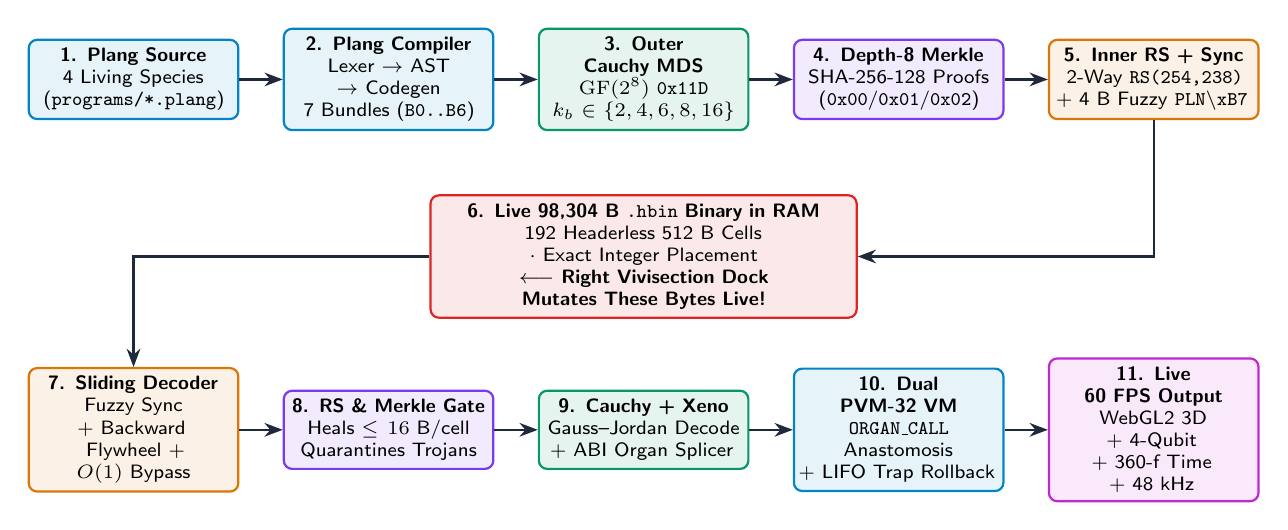
\begin{tikzpicture}[
  font=\scriptsize\sffamily,
  >=Stealth,
  node distance=4.5mm and 5.5mm,
  box/.style={draw=#1, fill=#1!10, rounded corners=3pt, thick, minimum height=9.5mm, text width=24.5mm, align=center, inner sep=3pt},
  widebox/.style={draw=#1, fill=#1!10, rounded corners=3pt, thick, minimum height=9mm, text width=36mm, align=center, inner sep=3pt},
  arr/.style={->, thick, draw=plnSlate}
]
  % Row 1: Build & Encode Pipeline
  \node[box=plnCyan]    (src)    {\textbf{1. Plang Source}\\4 Living Species\\(\texttt{programs/*.plang})};
  \node[box=plnCyan, right=of src]    (cmp)    {\textbf{2. Plang Compiler}\\Lexer $\to$ AST $\to$ Codegen\\7 Bundles (\texttt{B0..B6})};
  \node[box=plnEmerald, right=of cmp] (cauchy) {\textbf{3. Outer Cauchy MDS}\\$\mathrm{GF}(2^8)$ \texttt{0x11D}\\$k_b\in\{2,4,6,8,16\}$};
  \node[box=plnViolet, right=of cauchy] (merkle) {\textbf{4. Depth-8 Merkle}\\SHA-256-128 Proofs\\(\texttt{0x00}/\texttt{0x01}/\texttt{0x02})};
  \node[box=plnGold, right=of merkle] (rs)     {\textbf{5. Inner RS + Sync}\\2-Way \texttt{RS(254,238)}\\+ 4~B Fuzzy \texttt{PLN\textbackslash xB7}};

  % Row 2: Holographic Binary & Live Vivisection
  \node[widebox=plnCrimson, below=8mm of cauchy, text width=52mm] (hbin) {\textbf{6. Live 98,304~B \texttt{.hbin} Binary in RAM}\\192 Headerless 512~B Cells $\cdot$ Exact Integer Placement\\$\longleftarrow$ \textbf{Right Vivisection Dock Mutates These Bytes Live!}};

  % Row 3: Decode & Execution Engines (anchored cleanly below hbin to guarantee zero overlap)
  \node[box=plnEmerald, below=9mm of hbin]  (inv)  {\textbf{9. Cauchy + Xeno}\\Gauss--Jordan Decode\\+ ABI Organ Splicer};
  \node[box=plnViolet, left=of inv]         (imm)  {\textbf{8. RS \& Merkle Gate}\\Heals $\le 16$~B/cell\\Quarantines Trojans};
  \node[box=plnGold, left=of imm]           (sync) {\textbf{7. Sliding Decoder}\\Fuzzy Sync + Backward\\Flywheel + $O(1)$ Bypass};
  \node[box=plnCyan, right=of inv]          (vm)   {\textbf{10. Dual PVM-32 VM}\\\texttt{ORGAN\_CALL} Anastomosis\\+ LIFO Trap Rollback};
  \node[box=plnMagenta, right=of vm]        (out)  {\textbf{11. Live 60~FPS Output}\\WebGL2 3D + 4-Qubit\\+ 360-f Time + 48~kHz};

  \draw[arr] (src) -- (cmp);
  \draw[arr] (cmp) -- (cauchy);
  \draw[arr] (cauchy) -- (merkle);
  \draw[arr] (merkle) -- (rs);
  \draw[arr] (rs.south) |- (hbin.east);
  \draw[arr] (hbin.west) -| (sync.north);
  \draw[arr] (sync) -- (imm);
  \draw[arr] (imm) -- (inv);
  \draw[arr] (inv) -- (vm);
  \draw[arr] (vm) -- (out);
\end{tikzpicture}
\caption[End-to-End PLANARIA v2.4.0 Compilation, Vivisection, Decoding \& Execution Pipeline]{Complete end-to-end PLANARIA v2.4.0 compilation, holographic encoding, live byte-level vivisection, decoding, virtual machine execution, and 3D/audio output pipeline.}
\label{fig:arch-pipeline}
\end{figure}

\subsection{The Four Compiled Living \texttt{.hbin} Species}
\label{sec:species}

Every time you select a species from the top dropdown, PLANARIA loads its real compiled 98,304-byte \texttt{.hbin} binary alongside an identical traditional monolithic control twin (\texttt{LINBIN01}). All four species share the unified Shared-Memory World-State ABI (\texttt{MEM[0..511]}), enabling cross-species organ transplants between any pair.

\begin{table}[ht]
\centering
\caption{The Four Compiled Living \texttt{.hbin} Species Loaded Live in PLANARIA v2.4.0.}
\label{tab:species}
\footnotesize
\begin{tabularx}{\textwidth}{@{} L{3.0cm} r r L{2.4cm} Y @{}}
\toprule
\textbf{Species (\texttt{.hbin})} & \textbf{Insns} & \textbf{Code B} & \textbf{Root / SHA-256} & \textbf{Interactive Role \& Stratum Degradation (S3 $\to$ S2 $\to$ S1 $\to$ S0)} \\
\midrule
\texttt{QUANTUM\_CHRONICLE} (Default) & 426 & 1,704 & \texttt{917d90dc...} \texttt{d41408ce...} & Flagship 3D Chrono-Quantum holographic driver coupling \texttt{PVM-32} telemetry, 4-qubit gate schedules, Bell/GHZ pulses, Chrono-Well dilation, and 4-voice harmonic PolyBLEP audio. \\
\texttt{AEGIS\_DRIFT} & 1,000 & 4,000 & \texttt{4f72e7e2...} \texttt{12b1e3eb...} & Playable 60~FPS neon vector starfighter arcade (WASD/Arrows + Space or Autopilot). S3: Starfield + shrapnel + shield halo + 4-voice synthwave $\to$ S2: Vector sprites $\to$ S1: Radar wireframe $\to$ S0: Ghost distress triangle + 1-bit heartbeat. \\
\texttt{SYNTH\_REACTOR} & 645 & 2,580 & \texttt{863ac05d...} \texttt{63dbacf6...} & 4-voice Lydian polyphonic FM/subtractive synthesizer \& phosphor-trailed Lissajous oscilloscope. Arrows bend frequency ratios. S3: Rings + 8-band spectrum + chords $\to$ S2: Lissajous plasma web $\to$ S1: Green scope grid $\to$ S0: Pulse ring. \\
\texttt{CIPHER\_VAULT} & 534 & 2,136 & \texttt{47dae7cb...} \texttt{95f8e053...} & 12-lane 32-bit ARX stream-cipher \& cryptographic avalanche bit-matrix workstation with pentatonic keystream audio. S3: Lock ring + entropy ribbon $\to$ S2: 12$\times$8 bit-matrix $\to$ S1: Parity bars $\to$ S0: Emergency lockdown cross. \\
\bottomrule
\end{tabularx}
\end{table}

\clearpage
% ============================================================================
% SECTION 2: COMPLETE VISUAL GUI ANATOMY & TOP BAR
% ============================================================================
\section{Complete Visual GUI Anatomy \& Top Header Bar}
\label{sec:gui-anatomy}

Figure~\ref{fig:studio-screenshot} shows the live PLANARIA Studio interface, and Figure~\ref{fig:gui-wireframe} maps every single screen region (\textbf{Zones A--H}) so you can locate any widget instantly.

\begin{figure}[ht]
\centering
\fboxsep=2pt
\fbox{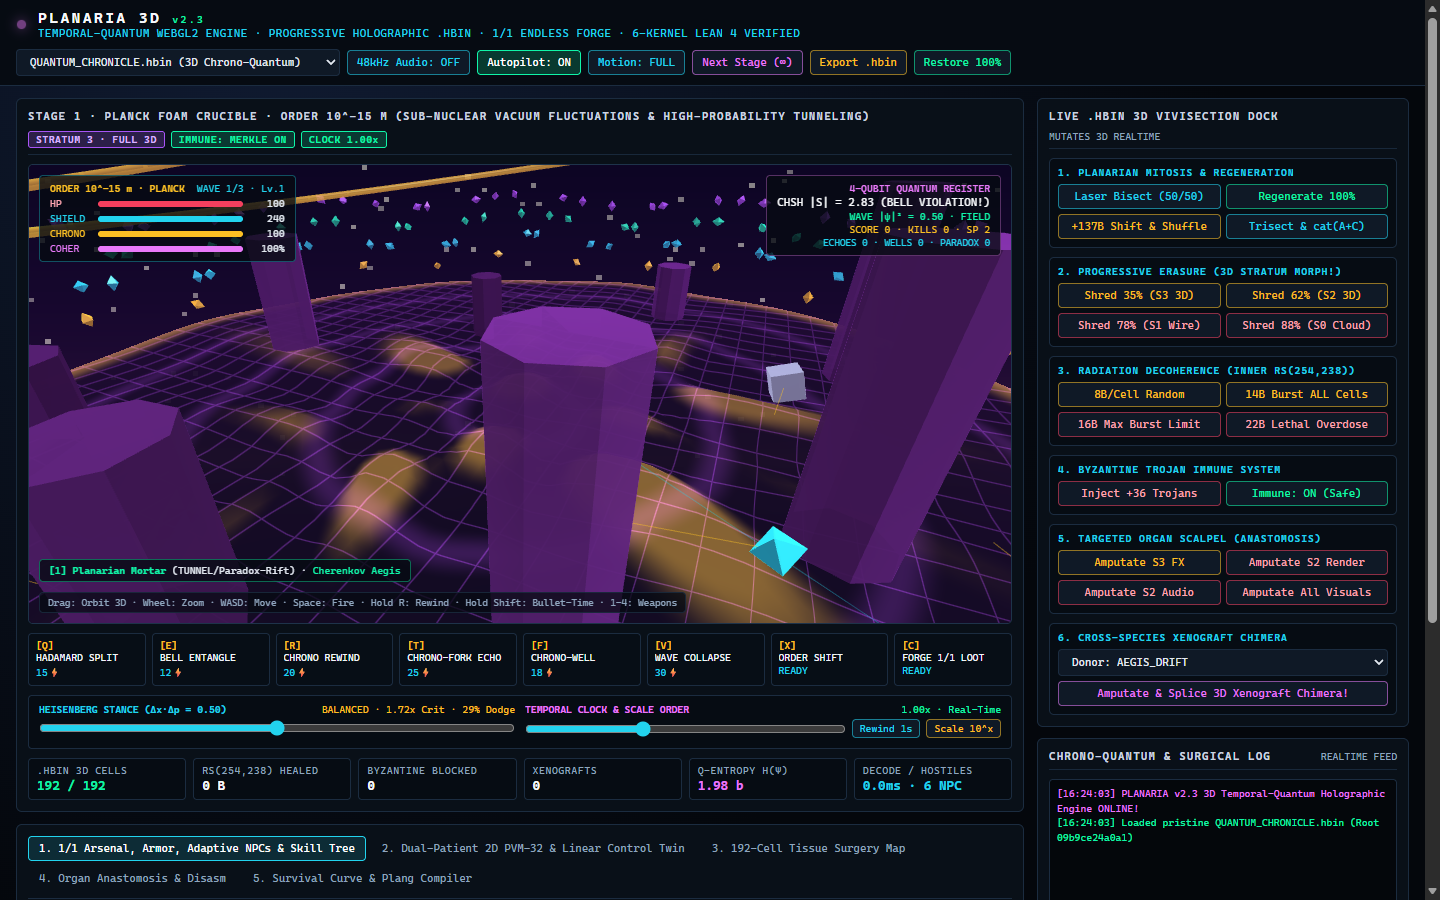
\includegraphics[width=0.94\textwidth]{../docs/media/studio-v2-3.png}}
\caption[Live PLANARIA 3D Temporal-Quantum Studio Viewport]{Live PLANARIA 3D Temporal-Quantum Holographic Engine \& Surgical Vivisection Studio viewport (captured from live Studio session; \texttt{v2.4.0} adds the \texttt{PROOF BLUEPRINT} link in Zone~A) showing the WebGL2 arena, top-left vitality HUD, top-right 4-qubit telemetry HUD, 8-ability bar, Heisenberg \& Temporal sliders, 6-box telemetry strip, Tab~1 RPG Forge, and Right-Hand Vivisection Dock.}
\label{fig:studio-screenshot}
\end{figure}

\begin{figure}[ht]
\centering
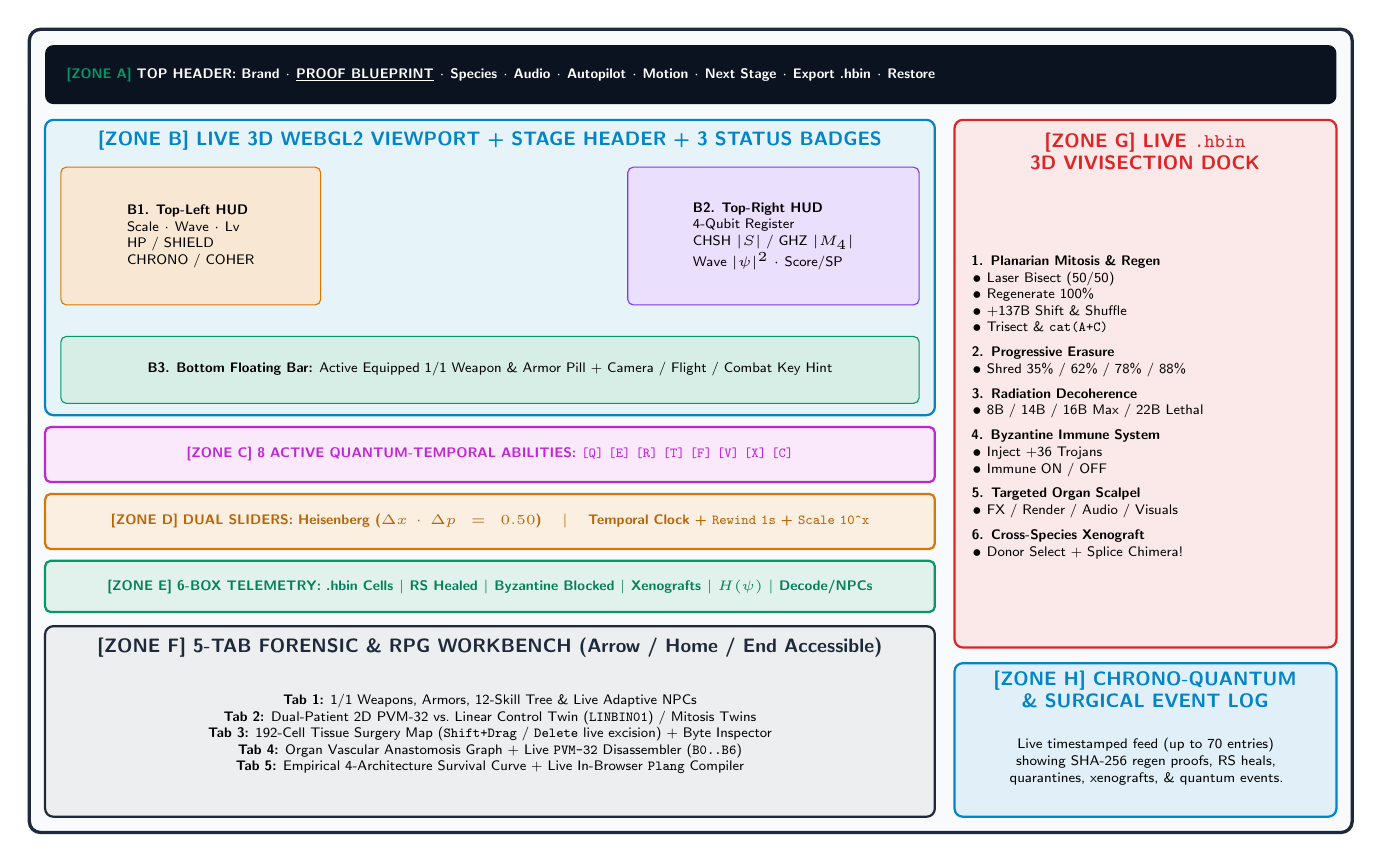
\begin{tikzpicture}[font=\scriptsize\sffamily]
  % Outer screen frame
  \draw[plnSlate, line width=1.2pt, rounded corners=4pt, fill=plnSoft] (0,0) rectangle (16.8,10.2);

  % Zone A: Top Header Bar
  \fill[plnBg, rounded corners=3pt] (0.2,9.25) rectangle (16.6,10.0);
  \node[text=white, anchor=west, font=\tiny\sffamily\bfseries] at (0.35,9.62) {\textbf{\color{plnEmerald}[ZONE A]} TOP HEADER: Brand $\cdot$ \underline{PROOF BLUEPRINT} $\cdot$ Species $\cdot$ Audio $\cdot$ Autopilot $\cdot$ Motion $\cdot$ Next Stage $\cdot$ Export .hbin $\cdot$ Restore};

  % Zone B: 3D Viewport
  \fill[plnCyan!10, draw=plnCyan, thick, rounded corners=3pt] (0.2,5.3) rectangle (11.5,9.05);
  \node[text=plnCyan, font=\scriptsize\sffamily\bfseries] at (5.85,8.78) {\textbf{[ZONE B]} LIVE 3D WEBGL2 VIEWPORT + STAGE HEADER + 3 STATUS BADGES};
  % Floating HUDs inside Zone B
  \fill[plnGold!18, draw=plnGold, rounded corners=2pt] (0.4,6.7) rectangle (3.7,8.45);
  \node[align=left, font=\tiny\sffamily] at (2.05,7.57) {\textbf{B1. Top-Left HUD}\\Scale $\cdot$ Wave $\cdot$ Lv\\HP / SHIELD\\CHRONO / COHER};
  \fill[plnViolet!16, draw=plnViolet, rounded corners=2pt] (7.6,6.7) rectangle (11.3,8.45);
  \node[align=left, font=\tiny\sffamily] at (9.45,7.57) {\textbf{B2. Top-Right HUD}\\4-Qubit Register\\CHSH $|S|$ / GHZ $|M_4|$\\Wave $|\psi|^2$ $\cdot$ Score/SP};
  \fill[plnEmerald!16, draw=plnEmerald, rounded corners=2pt] (0.4,5.45) rectangle (11.3,6.3);
  \node[align=center, font=\tiny\sffamily] at (5.85,5.88) {\textbf{B3. Bottom Floating Bar:} Active Equipped 1/1 Weapon \& Armor Pill + Camera / Flight / Combat Key Hint};

  % Zone C: 8 Abilities
  \fill[plnMagenta!10, draw=plnMagenta, thick, rounded corners=2pt] (0.2,4.45) rectangle (11.5,5.15);
  \node[text=plnMagenta, font=\tiny\sffamily\bfseries, text width=10.9cm, align=center] at (5.85,4.80) {\textbf{[ZONE C]} 8 ACTIVE QUANTUM-TEMPORAL ABILITIES: \texttt{[Q] [E] [R] [T] [F] [V] [X] [C]}};

  % Zone D: Sliders
  \fill[plnGold!12, draw=plnGold, thick, rounded corners=2pt] (0.2,3.6) rectangle (11.5,4.3);
  \node[text=plnGold!85!black, font=\tiny\sffamily\bfseries, text width=10.9cm, align=center] at (5.85,3.95) {\textbf{[ZONE D]} DUAL SLIDERS: Heisenberg ($\Delta x\cdot\Delta p=0.50$) $\;\vert\;$ Temporal Clock + \texttt{Rewind 1s} + \texttt{Scale 10\^{}x}};

  % Zone E: 6-Box Telemetry Strip
  \fill[plnEmerald!12, draw=plnEmerald, thick, rounded corners=2pt] (0.2,2.8) rectangle (11.5,3.45);
  \node[text=plnEmerald!85!black, font=\tiny\sffamily\bfseries, text width=10.9cm, align=center] at (5.85,3.12) {\textbf{[ZONE E]} 6-BOX TELEMETRY: .hbin Cells $\vert$ RS Healed $\vert$ Byzantine Blocked $\vert$ Xenografts $\vert$ $H(\psi)$ $\vert$ Decode/NPCs};

  % Zone F: 5-Tab Workbench
  \fill[plnSlate!8, draw=plnSlate, thick, rounded corners=3pt] (0.2,0.2) rectangle (11.5,2.62);
  \node[text=plnSlate, font=\scriptsize\sffamily\bfseries] at (5.85,2.35) {\textbf{[ZONE F]} 5-TAB FORENSIC \& RPG WORKBENCH (Arrow / Home / End Accessible)};
  \node[align=center, font=\tiny\sffamily] at (5.85,1.25) {\textbf{Tab 1:} 1/1 Weapons, Armors, 12-Skill Tree \& Live Adaptive NPCs\\
    \textbf{Tab 2:} Dual-Patient 2D PVM-32 vs.\ Linear Control Twin (\texttt{LINBIN01}) / Mitosis Twins\\
    \textbf{Tab 3:} 192-Cell Tissue Surgery Map (\texttt{Shift+Drag} / \texttt{Delete} live excision) + Byte Inspector\\
    \textbf{Tab 4:} Organ Vascular Anastomosis Graph + Live \texttt{PVM-32} Disassembler (\texttt{B0..B6})\\
    \textbf{Tab 5:} Empirical 4-Architecture Survival Curve + Live In-Browser \texttt{Plang} Compiler};

  % Zone G: Right Vivisection Dock
  \fill[plnCrimson!10, draw=plnCrimson, thick, rounded corners=3pt] (11.75,2.35) rectangle (16.6,9.05);
  \node[text=plnCrimson, font=\scriptsize\sffamily\bfseries, align=center] at (14.17,8.65) {\textbf{[ZONE G]} LIVE \texttt{.hbin}\\3D VIVISECTION DOCK};
  \node[align=left, font=\tiny\sffamily, text width=4.4cm] at (14.17,5.4) {%
    \textbf{1. Planarian Mitosis \& Regen}\\
    $\bullet$ Laser Bisect (50/50)\\
    $\bullet$ Regenerate 100\%\\
    $\bullet$ +137B Shift \& Shuffle\\
    $\bullet$ Trisect \& \texttt{cat(A+C)}\\[3pt]
    \textbf{2. Progressive Erasure}\\
    $\bullet$ Shred 35\% / 62\% / 78\% / 88\%\\[3pt]
    \textbf{3. Radiation Decoherence}\\
    $\bullet$ 8B / 14B / 16B Max / 22B Lethal\\[3pt]
    \textbf{4. Byzantine Immune System}\\
    $\bullet$ Inject +36 Trojans\\
    $\bullet$ Immune ON / OFF\\[3pt]
    \textbf{5. Targeted Organ Scalpel}\\
    $\bullet$ FX / Render / Audio / Visuals\\[3pt]
    \textbf{6. Cross-Species Xenograft}\\
    $\bullet$ Donor Select + Splice Chimera!};

  % Zone H: Realtime Log
  \fill[plnCyan!12, draw=plnCyan, thick, rounded corners=3pt] (11.75,0.2) rectangle (16.6,2.15);
  \node[text=plnCyan, font=\scriptsize\sffamily\bfseries, align=center] at (14.17,1.82) {\textbf{[ZONE H]} CHRONO-QUANTUM\\\& SURGICAL EVENT LOG};
  \node[align=center, font=\tiny\sffamily, text width=4.4cm] at (14.17,0.9) {Live timestamped feed (up to 70 entries) showing SHA-256 regen proofs, RS heals, quarantines, xenografts, \& quantum events.};
\end{tikzpicture}
\caption[Annotated GUI Wireframe Map (Zones A--H)]{Annotated GUI Wireframe Map showing every interactive zone (\textbf{Zones A--H}) of the PLANARIA v2.4 Studio.}
\label{fig:gui-wireframe}
\end{figure}

\clearpage
\subsection{Zone A --- Top Header Bar Reference (Every Control)}
\label{sec:zone-a}

\begin{table}[ht]
\centering
\caption{Complete Reference for Zone A (Top Header Bar Controls).}
\label{tab:zone-a}
\footnotesize
\begin{tabularx}{\textwidth}{@{} L{3.3cm} L{2.8cm} Y @{}}
\toprule
\textbf{Control / Element} & \textbf{Default State} & \textbf{Exact Function \& Underlying Behavior} \\
\midrule
Pulsing Emerald Dot + \texttt{PLANARIA 3D v2.4} & Active & Visual heartbeat indicator and version label (\texttt{VERSION = 2.4.0}). \\
\texttt{PROOF BLUEPRINT} link & Link (\texttt{./blueprint/}) & Opens the interactive Lean~4.35.0 Proof Dependency Blueprint (Section~\ref{sec:blueprint}), displaying all 85 audited theorems, 18 intra-proof dependency edges, axiom allowlists, and source signatures. \\
\textbf{Species Selector} (\texttt{\#speciesSelect}) & \texttt{QUANTUM\_CHRONICLE} & Switches active compiled 98,304~B \texttt{.hbin} species (\texttt{QUANTUM\_CHRONICLE}, \texttt{AEGIS\_DRIFT}, \texttt{SYNTH\_REACTOR}, or \texttt{CIPHER\_VAULT}). Resets \texttt{currentBytes}, rebuilds the matching \texttt{LINBIN01} control twin, pins \texttt{pinnedRootHex}, populates the Tab~5 \texttt{Plang} editor, updates the Donor dropdown to a different species, and reboots \texttt{PVM-32}. \\
\texttt{48kHz Audio: OFF / ON} & \texttt{OFF} (\texttt{aria-pressed}) & Initializes or mutes the lock-free 48~kHz 4-voice PolyBLEP \texttt{AudioWorklet} synth (\texttt{src/web/audio-worklet.js}). Directly driven by Bundle~4 (\texttt{S2\_SYNTH\_AUDIO}); amputating or xenografting Bundle~4 changes live audio instantaneously. \\
\texttt{Autopilot: ON / OFF} & \texttt{ON} & Toggles autonomous AI piloting of the player avatar in both the 3D WebGL2 arena and the 2D \texttt{PVM-32} game. Turn \texttt{OFF} to fly, strafe, and shoot manually. \\
\texttt{Motion: FULL / REDUCED} & \texttt{FULL} (or OS pref) & Accessibility control (automatically enabled when OS \texttt{prefers-reduced-motion: reduce} is set). Dampens particle bursts, disables aggressive animations, and pauses autopilot. \\
\texttt{Next Stage ($\infty$)} & Button & Advances to the next procedural stage (\texttt{Stage 1 $\to$ 2 $\to$ $\dots$ $\infty$}), cycling across the 6 Scale Realms with new procedural monolith pillars, multi-slit wave sources, escalating waves, and tougher Singularity Archon bosses. \\
\texttt{Export .hbin} & Button & Downloads the exact live byte buffer in RAM (\texttt{98,304 B} pristine/healed/chimera, or exact damaged/bisected shard length) as \texttt{<species>\_live.hbin} or \texttt{<species>\_chimera.hbin}, ready to inspect or run via \texttt{node bin/planaria.mjs}. \\
\texttt{Restore 100\%} & Button & Immediately reloads the pristine 192/192-cell binary of the current species, restores the Control Twin, re-pins the lineage root, and clears Mitosis/Xenograft modes. \\
\bottomrule
\end{tabularx}
\end{table}

\FloatBarrier
% ============================================================================
% SECTION 3: 3D VIEWPORT, STATUS BADGES, HUD METERS & CONTROLS
% ============================================================================
\section{Zone B --- Live 3D WebGL2 Viewport, Status Badges, HUDs \& Controls}
\label{sec:zone-b}

The 3D viewport is rendered by a custom zero-dependency \textbf{WebGL2 (\texttt{GLSL 300 es})} engine (\path{src/web/renderer3d.js}) with outward counter-clockwise procedural meshes, CPU inverse-transpose normal matrices, deduplicated wireframe element buffers, GPU-evaluated multi-source Schr\"odinger floor waves, and graceful \texttt{webglcontextlost} fallback (if WebGL2 is unavailable, a clear status banner appears and all 2D \texttt{PVM-32}, Tissue Surgery, and Audio features keep running uninterrupted).

\subsection{Live Visual Elements Inside the 3D Scene}
\begin{itemize}[leftmargin=1.5em, itemsep=1.5pt]
  \item \textbf{192 Orbiting Holographic Cell Crystals:} Every physical 512-byte cell of your live \texttt{.hbin} file orbits above the arena in a double-helix ring colored by bundle stratum and live status (gold/cyan/emerald/purple for intact, amber for RS-repaired, crimson for quarantined, magenta for xenografted, vanished when erased!).
  \item \textbf{Multi-Slit Wave Interference Floor:} The glowing arena floor evaluates $|\sum_k A_k e^{i(k r - \omega t + \phi_k)}|^2$ live across 3--5 stage emitters. Bright ridges represent constructive interference peaks ($|\psi|^2 > 1.35 \implies 2.2\times$ damage boost).
  \item \textbf{WKB Tunneling Monoliths:} Procedural 3D pillars around the perimeter each carry a barrier potential $V_0 \in [0.4, 1.6]$. Standard shots stop at pillars; weapons with high \texttt{tunnelFactor} or \texttt{WKB Tunneling} pass straight through them (and \texttt{Barrier Resonance} boosts post-tunnel shots by $+80\%$!).
  \item \textbf{Quantum \& Temporal Visual Effects:} Twin translucent cyan clones during \texttt{HADAMARD SPLIT}, glowing magenta tethers linking Bell/GHZ-entangled enemies, translucent amber \texttt{Chrono-Wells} visibly slowing enemy motion inside, glowing past-self \texttt{Echo Clones} retracing your last 4~seconds, and faint retrocausal future-cone prediction lines.
\end{itemize}

\begin{figure}[ht]
\centering
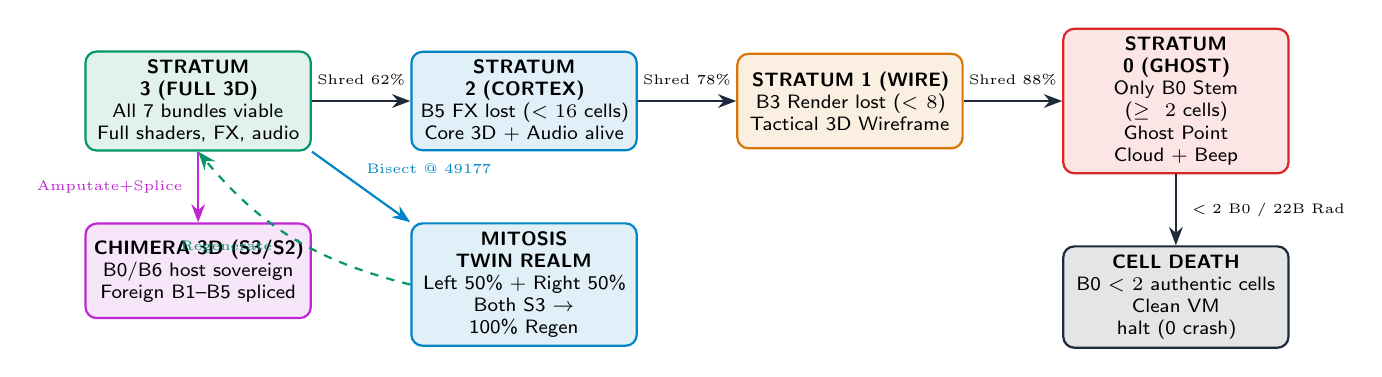
\begin{tikzpicture}[
  font=\scriptsize\sffamily,
  >=Stealth,
  state/.style={draw=#1, fill=#1!12, rounded corners=4pt, thick, minimum height=12mm, text width=26.5mm, align=center, inner sep=3pt},
  arr/.style={->, thick, draw=plnSlate}
]
  \node[state=plnEmerald] (s3) {\textbf{STRATUM 3 (FULL 3D)}\\All 7 bundles viable\\Full shaders, FX, audio};
  \node[state=plnCyan, right=12.5mm of s3] (s2) {\textbf{STRATUM 2 (CORTEX)}\\B5 FX lost ($<16$ cells)\\Core 3D + Audio alive};
  \node[state=plnGold, right=12.5mm of s2] (s1) {\textbf{STRATUM 1 (WIRE)}\\B3 Render lost ($<8$)\\Tactical 3D Wireframe};
  \node[state=plnCrimson, right=12.5mm of s1] (s0) {\textbf{STRATUM 0 (GHOST)}\\Only B0 Stem ($\ge 2$ cells)\\Ghost Point Cloud + Beep};
  \node[state=plnSlate, below=9mm of s0] (dead) {\textbf{CELL DEATH}\\B0 $< 2$ authentic cells\\Clean VM halt (0 crash)};
  \node[state=plnMagenta, below=9mm of s3] (xeno) {\textbf{CHIMERA 3D (S3/S2)}\\B0/B6 host sovereign\\Foreign B1--B5 spliced};
  \node[state=plnCyan, below=9mm of s2] (mito) {\textbf{MITOSIS TWIN REALM}\\Left 50\% + Right 50\%\\Both S3 $\to$ 100\% Regen};

  \draw[arr] (s3) -- node[above=2pt, font=\tiny]{Shred 62\%} (s2);
  \draw[arr] (s2) -- node[above=2pt, font=\tiny]{Shred 78\%} (s1);
  \draw[arr] (s1) -- node[above=2pt, font=\tiny]{Shred 88\%} (s0);
  \draw[arr] (s0) -- node[right=2pt, font=\tiny]{$<2$ B0 / 22B Rad} (dead);
  \draw[arr, plnMagenta] (s3) -- node[left=2pt, font=\tiny]{Amputate+Splice} (xeno);
  \draw[arr, plnCyan] (s3.south east) -- node[above right, font=\tiny, pos=0.45]{Bisect @ 49177} (mito.north west);
  \draw[arr, plnEmerald, dashed] (mito.west) to[bend left=18] node[below left, font=\tiny, pos=0.55]{Regenerate} (s3.south);
\end{tikzpicture}
\caption[Live 3D Stratum Visual Metamorphosis State Machine]{Live 3D Stratum Visual Metamorphosis State Machine driven directly by \texttt{.hbin} bundle rank survival.}
\label{fig:stratum-morph}
\end{figure}

\clearpage
\subsection{Status Badges \& Floating HUD Readouts (Zones B1, B2, B3)}

\begin{table}[!ht]
\centering
\caption{Complete Reference for Every Status Badge and Floating HUD Readout Inside Zone B.}
\label{tab:zone-b-hud}
\footnotesize
\begin{tabularx}{\textwidth}{@{} L{3.6cm} L{2.3cm} Y @{}}
\toprule
\textbf{HUD Element} & \textbf{Location} & \textbf{Exact Data Meaning \& Trigger Conditions} \\
\midrule
Stage Header Title & Top-Left of Panel & Shows \texttt{STAGE N $\cdot$ <REALM NAME> (TIER C) $\cdot$ ORDER 10\^{}x (<Subtitle>)}. Updates live on \texttt{Next Stage} or \texttt{Scale 10\^{}x}. \\
\pill{plnEmerald}{STRATUM 3 $\cdot$ FULL 3D} & Top-Right Badge 1 & Active binary capability level: \texttt{STRATUM 3}, \texttt{STRATUM 2}, \texttt{STRATUM 1}, \texttt{STRATUM 0}, \texttt{CHIMERA 3D $\cdot$ Sx} (magenta), or \texttt{CELL DEATH} (red). \\
\pill{plnCyan}{IMMUNE: MERKLE ON} & Top-Right Badge 2 & Reflects whether Depth-8 SHA-256 Merkle quarantine is actively blocking forged cells. Turns crimson \texttt{IMMUNE: OFF (UNSAFE!)} if toggled off in Dock Group~4. \\
\pill{plnGold}{CLOCK 1.00x} & Top-Right Badge 3 & Live temporal speed: \texttt{CLOCK <v>x} (normal/haste), \texttt{BULLET-TIME <v>x} ($<0.5\times$), or \texttt{$\blacktriangleleft\blacktriangleleft$ REWINDING TIME} during reverse scrubbing. \\
\texttt{ORDER 10\^{}x $\cdot$ WAVE W/3 $\cdot$ Lv.L} & Zone B1 (Top-Left) & Current logarithmic scale label, wave progress (Waves 1--2 are squads; Wave~3 spawns a Stage Singularity Archon Boss), and player RPG level (gaining levels awards $+1$ Skill Point). \\
\texttt{HP} Meter (Red) & Zone B1 & Current / max hull hit points (starts at \texttt{100/100}). Fully restored along with past positions when rewinding time via \kbd{R}. \\
\texttt{SHIELD} Meter (Cyan) & Zone B1 & Energy shield pool determined by equipped 1/1 Armor (\texttt{maxShield} and \texttt{regenRate}/s), scaled by \texttt{RS(254,238) Autophagy} skill and Heisenberg \texttt{shieldDensity}. \\
\texttt{CHRONO} Meter (Gold) & Zone B1 & Temporal energy pool (\texttt{0..100}) powering \kbd{Q}/\kbd{E}/\kbd{R}/\kbd{T}/\kbd{F}/\kbd{V} and \kbd{Shift} bullet-time. Regenerates passively, boosted by \texttt{Chronon Capacitor} armor and \texttt{Entropy-Rewind} weapon hits. \\
\texttt{COHER} Meter (Magenta) & Zone B1 & Quantum visibility $V \in [0\%, 100\%]$ of the 4-qubit Werner state $\rho = V|\psi\rangle\langle\psi| + (1-V)I/16$. Decays when \texttt{.hbin} radiation bursts hit (unless wearing \texttt{Merkle Byzantine Barrier} armor), reducing CHSH/GHZ nonlocality until regenerated. \\
\texttt{CHSH |S|} / \texttt{GHZ |M\_4|} & Zone B2 (Top-Right) & Exact Bell/Mermin nonlocality readout computed live from the 16 complex amplitudes. Displays \texttt{(BELL VIOLATION!)} whenever $|S| > 2.005$ (Tsirelson max $2\sqrt{2}\approx 2.83$), or \texttt{GHZ |M\_4| = 4.00 (NON-LOCAL!)} during 4-qubit GHZ entanglement. \\
\texttt{WAVE} $|\psi|^2$ & Zone B2 & Multi-slit floor wave intensity at player coordinates. Displays \texttt{CONSTRUCTIVE 2.2x!} when standing on a bright ridge ($|\psi|^2 > 1.35$). \\
\texttt{SCORE $\cdot$ KILLS $\cdot$ SP} & Zone B2 & Total combat score, enemies defeated, and unspent Skill Points (starts at \texttt{2 SP}). \\
\texttt{ECHOES $\cdot$ WELLS $\cdot$ PARADOX} & Zone B2 & Active Past-Timeline Echo Clones, active 3D Chrono-Wells, and cumulative temporal paradox count. \\
Equipped Loadout Pill & Zone B3 (Bottom-Left) & Color-coded summary of active weapon slot \texttt{[1--4]}, Quantum/Temporal mod tags, and active armor short name. \\
\bottomrule
\end{tabularx}
\end{table}

\FloatBarrier
\subsection{Master Keyboard, Mouse \& Accessibility Controls Card}
\label{sec:controls}

\begin{table}[!ht]
\centering
\caption[Keyboard, Pointer \& Accessibility Controls]{Complete Keyboard, Pointer, and Accessibility Control Reference (Layout-Independent Physical Key Codes).}
\label{tab:controls}
\footnotesize
\begin{tabularx}{\textwidth}{@{} L{3.8cm} L{2.8cm} Y @{}}
\toprule
\textbf{Input / Shortcut} & \textbf{Scope} & \textbf{Exact Action} \\
\midrule
\kbd{Mouse Drag} or \kbd{J} \kbd{L} \kbd{I} \kbd{K} & 3D Viewport & Orbit camera yaw (\kbd{J}/\kbd{L}) and pitch (\kbd{I}/\kbd{K}, clamped $[0.14, 1.42]$ rad). \\
\kbd{Mouse Wheel} or \kbd{+} \kbd{-} & 3D Viewport & Zoom camera distance smoothly between \texttt{11} and \texttt{64} world units. \\
\kbd{W} \kbd{A} \kbd{S} \kbd{D} or Arrow Keys & Arena & Move player relative to current 3D camera yaw (also drives 2D \texttt{PVM-32} game when Autopilot is OFF). \\
\kbd{Space} & Arena & Fire equipped 1/1 weapon (smartly suppressed when keyboard focus is on a button/tab/editor!). \\
\kbd{Hold R} & Temporal Engine & Continuously scrub the entire 3D universe backwards through the 360-frame \texttt{RingBuffer}. \\
\kbd{Hold Shift} & Temporal Engine & Engage Bullet-Time slow motion while held. \\
\kbd{1} \kbd{2} \kbd{3} \kbd{4} & Arsenal & Instantly equip Weapon Slot 1, 2, 3, or 4. \\
\kbd{Q} \kbd{E} \kbd{T} \kbd{F} \kbd{V} \kbd{X} \kbd{C} & Ability Bar & Trigger active Quantum-Temporal Abilities (Table~\ref{tab:abilities}). \\
\kbd{Tab} / \kbd{$\leftarrow$} \kbd{$\rightarrow$} \kbd{Home} \kbd{End} & Workbench Tabs & Full WAI-ARIA roving-tabindex navigation across Tabs 1--5 without moving the 3D player. \\
\kbd{Click} / \kbd{Arrows} (Tab~3) & Tissue Surgery Map & Select any of the 192 cells to inspect raw 512-byte anatomy. \\
\kbd{Shift+Drag} / \kbd{Del} (Tab~3) & Tissue Surgery Map & Surgically zero/destroy cells live under your cursor or keyboard focus. \\
\bottomrule
\end{tabularx}
\end{table}

\FloatBarrier
% ============================================================================
% SECTION 4: QUANTUM MECHANICS, TEMPORAL ENGINE, ABILITIES & SLIDERS
% ============================================================================
\section{Zones C \& D --- Quantum Mechanics, Temporal Engine, 8 Abilities \& Sliders}
\label{sec:quantum-temporal}

\subsection{Zone C --- The 8 Active Quantum-Temporal Abilities}

\begin{table}[ht]
\centering
\caption{Complete Reference for All 8 Active Quantum-Temporal Abilities (Zone C Action Bar).}
\label{tab:abilities}
\footnotesize
\begin{tabularx}{\textwidth}{@{} c L{3.0cm} c c Y @{}}
\toprule
\textbf{Key} & \textbf{Ability Name} & \textbf{Cost (CE)} & \textbf{CD} & \textbf{Exact Quantum / Temporal Mechanic \& Combat Effect} \\
\midrule
\kbd{Q} & \textbf{HADAMARD SPLIT} & 15~\textsc{ce} & 5.0~s & Applies Hadamard gates $H$ to the 4-qubit register and splits your avatar into twin phase-interfering superposition clones for 4~seconds with double fire and 50\% probabilistic dodge. \\
\kbd{E} & \textbf{BELL ENTANGLE} & 12~\textsc{ce} & 4.5~s & Prepares a Bell/GHZ entangled web across qubits and links up to 4 nearest hostiles (more with \texttt{GHZ Multi-Body Web} skill). Damage dealt to any linked enemy echoes non-locally across all entangled partners (55\%--115\% via \texttt{Tsirelson Bell Link}). \\
\kbd{R} & \textbf{CHRONO REWIND} & 20~\textsc{ce} & 0.5~s & Click for a 45-frame pulse or \textbf{hold \kbd{R}} to scrub backwards up to 6.0~seconds (360 frames). Restores HP, shields, positions, projectiles, NPC states, 4-qubit amplitudes, skills, inventory, and PRNG state atomically. \\
\kbd{T} & \textbf{CHRONO-FORK ECHO} & 25~\textsc{ce} & 7.5~s & Forks your recorded player trail: spawns an autonomous glowing \textbf{Past Self} replaying your last 4~seconds of movement and weapon fire alongside you. \\
\kbd{F} & \textbf{CHRONO-WELL} & 18~\textsc{ce} & 6.0~s & Deploys a 3D translucent spherical time-dilation field slowing enemy movement and hostile bullets inside to $0.16\times$ speed (radius and depth boosted by \texttt{Chrono-Well Radius} skill). \\
\kbd{V} & \textbf{WAVE COLLAPSE} & 30~\textsc{ce} & 8.5~s & Performs an exact Born-rule projective measurement of the 4-qubit register, detonating an arena-wide collapse supernova whose damage scales with Shannon entropy $H(\psi)$ and CHSH violation $|S|$. \\
\kbd{X} & \textbf{ORDER SHIFT} & 0~\textsc{ce} & 1.5~s & Shifts the active \textbf{Scale Realm} across 6 logarithmic realms spanning 24 orders of magnitude ($10^{-15}\,\text{m} \to 10^9\,\text{m}$; Table~\ref{tab:realms}), updating atmosphere, tunneling boost, wave frequency, and harmonic musical mode live. \\
\kbd{C} & \textbf{FORGE 1/1 LOOT} & 0~\textsc{ce} & 2.0~s & Synthesizes a brand-new unique 1/1 Quantum Weapon \& Armor pair seeded from live SHA-256 entropy (\texttt{seed : lootSeq : worldTime : lineageRoot}). \\
\bottomrule
\end{tabularx}
\end{table}

\subsection{Exact Mathematical Models Powering the Quantum \& Temporal Engines}

All quantum telemetry displayed in Zone B2 and Zone E is computed by exact double-precision linear algebra in \texttt{src/quantum/qengine.js} (cross-checked in Python~3 by \texttt{reference/planaria\_oracle.py} and formally verified for $\mathbb{Z}[i]$ 4-qubit unitarity in \texttt{lean/PlanariaProofs/QuantumTemporal.lean}):

\begin{itemize}[leftmargin=1.5em, itemsep=2pt]
  \item \textbf{4-Qubit Complex Statevector ($|\psi\rangle \in \mathbb{C}^{16}$):} Stores 16 complex amplitudes with exact unitary gates \texttt{H, X, Y, Z, RX, RY, RZ, CNOT, CZ, SWAP}, exact Born-rule projective measurement honoring Werner visibility $V \in [0, 1]$ ($\rho = V|\psi\rangle\langle\psi| + (1-V)I/16$), purity $\operatorname{Tr}(\rho^2) = (1 + 15V^2)/16$, and computational-basis Shannon entropy $H(\psi) = -\sum_{i=0}^{15} p_i \log_2 p_i \in [0, 4]$ bits.
  \item \textbf{Horodecki CHSH Criterion (Rotation-Invariant Bell Correlator):} Forms the exact $3\times 3$ Pauli correlation tensor $T_{ab} = \langle \sigma_a^{(q_A)} \otimes \sigma_b^{(q_B)} \rangle$, solves the eigenvalues $\lambda_1 \ge \lambda_2 \ge \lambda_3$ of $M = T^\top T$ via 18-step cyclic Jacobi iteration, and evaluates
  \begin{equation}
    S_{\max} = 2\sqrt{\lambda_1 + \lambda_2}\cdot V \;\le\; 2\sqrt{2} \approx 2.828427,
  \end{equation}
  guaranteed $\le 2.0$ on every separable state and invariant under arbitrary local unitary rotations.
  \item \textbf{4-Qubit Mermin--Klyshko Nonlocality Correlator ($M_4$):} Evaluates the exact 8-term Pauli operator
  \begin{equation}
    M_4 = \tfrac{1}{2}\langle XXXX - XXYY - XYXY - XYYX - YXXY - YXYX - YYXX + YYYY\rangle \cdot V,
  \end{equation}
  bounded by $|M_4| \le 2.0$ classically and reaching $|M_4| = 4.0$ on the 4-qubit GHZ state $(|0000\rangle+|1111\rangle)/\sqrt{2}$.
  \item \textbf{WKB Tunneling \& Quantum Zeno Gaze:} Projectiles hitting a monolith of potential $V_0$ and width $d$ tunnel with probability $T(E,V_0,d) = \exp\!\bigl(-2d\sqrt{2m(V_0 - E)}\bigr)$ for $E < V_0$ (and $1.0$ for $E \ge V_0$). Enemies stared at directly by the camera sightline experience Quantum Zeno motion suppression $f_{\text{Zeno}} = \bigl(1 + (\nu \tau_Z)^2\bigr)^{-1}$.
\end{itemize}

\subsection{Zone D --- The Two Interactive Sliders (Exact Equations \& Trade-Off Curves)}

\begin{enumerate}[leftmargin=1.5em, itemsep=2pt]
  \item \textbf{Heisenberg Uncertainty Stance Slider ($s \in [0, 1]$, label \texttt{0..100}):} Saturates the minimum-uncertainty bound $\Delta x \cdot \Delta p = 0.50$ identically across the entire range via $\Delta x = 0.35 + 1.65s$ and $\Delta p = 0.50 / \Delta x$. Moving left (\textbf{Position-Lock}, $s < 0.35$) maximizes \textbf{aim precision} ($1.0 - 0.45s \to 1.00$) and \textbf{shield barrier density} ($1.55 - 0.75s \to 1.55\times$); moving right (\textbf{Momentum-Blur}, $s > 0.65$) maximizes \textbf{critical multiplier} ($1.0 + 1.45s \to 2.45\times$) and \textbf{probabilistic wavepacket dodge} ($0.58s \to 58\%$). Figure~\ref{fig:heisenberg-chart} plots every curve simultaneously.
  \item \textbf{Temporal Clock Slider (\texttt{0.15x} to \texttt{2.50x}) + Pulse Buttons:} Sets \nolinkurl{world.temporal.globalTimeScale} directly from extreme Time Dilation ($0.15\times$) through Real-Time ($1.00\times$) up to Hyper-Chronon ($2.50\times$). Click \textbf{\texttt{Rewind 1s}} for an instant 55-frame backward burst, or \textbf{\texttt{Scale 10\^{}x}} to cycle through the 6 Scale Realms (Table~\ref{tab:realms}).
\end{enumerate}

\begin{figure}[ht]
\centering
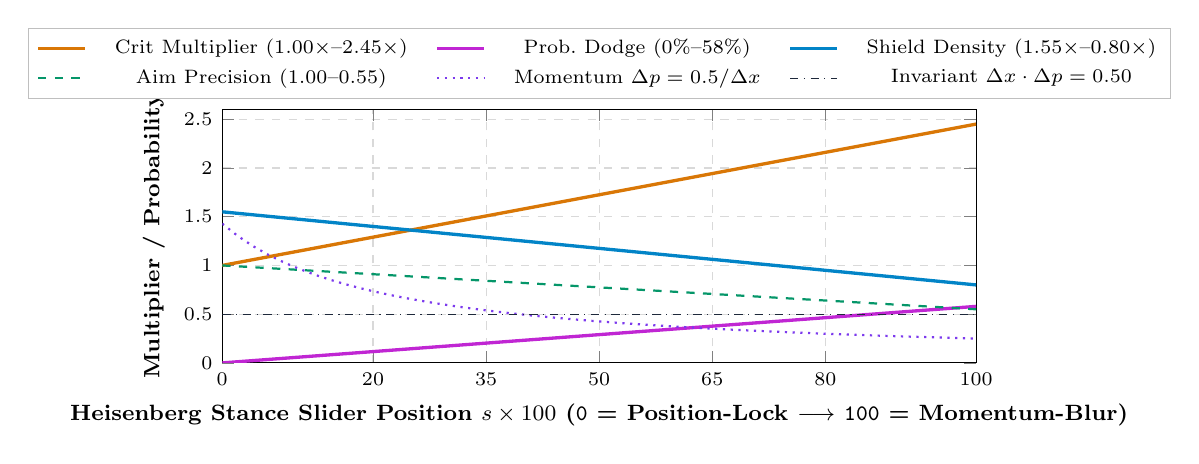
\begin{tikzpicture}
\begin{axis}[
  width=0.92\textwidth,
  height=4.8cm,
  xlabel={Heisenberg Stance Slider Position $s \times 100$ (\texttt{0} = Position-Lock $\longrightarrow$ \texttt{100} = Momentum-Blur)},
  ylabel={Multiplier / Probability},
  xmin=0, xmax=100,
  ymin=0, ymax=2.6,
  xtick={0,20,35,50,65,80,100},
  ytick={0,0.5,1.0,1.5,2.0,2.5},
  grid=major,
  grid style={dashed, gray!30},
  legend columns=3,
  legend style={at={(0.5,1.04)}, anchor=south, font=\scriptsize, fill=white, draw=gray!50, column sep=8pt},
  tick label style={font=\scriptsize},
  label style={font=\footnotesize\bfseries}
]
  \addplot[color=plnGold, very thick, domain=0:100, samples=50] {1.0 + 1.45*(x/100)};
  \addlegendentry{Crit Multiplier ($1.00\times$--$2.45\times$)}

  \addplot[color=plnMagenta, very thick, domain=0:100, samples=50] {0.58*(x/100)};
  \addlegendentry{Prob.\ Dodge (0\%--58\%)}

  \addplot[color=plnCyan, very thick, domain=0:100, samples=50] {1.55 - 0.75*(x/100)};
  \addlegendentry{Shield Density ($1.55\times$--$0.80\times$)}

  \addplot[color=plnEmerald, thick, dashed, domain=0:100, samples=50] {1.0 - 0.45*(x/100)};
  \addlegendentry{Aim Precision ($1.00$--$0.55$)}

  \addplot[color=plnViolet, thick, dotted, domain=0:100, samples=50] {0.5 / (0.35 + 1.65*(x/100))};
  \addlegendentry{Momentum $\Delta p = 0.5/\Delta x$}

  \addplot[color=plnSlate, thin, dashdotted, domain=0:100, samples=2] {0.5};
  \addlegendentry{Invariant $\Delta x\cdot\Delta p = 0.50$}
\end{axis}
\end{tikzpicture}
\caption[Exact Heisenberg Uncertainty Stance Curves (\texttt{heisenbergStance})]{Exact Heisenberg Uncertainty Stance curves (\texttt{heisenbergStance} in \texttt{src/quantum/qengine.js}).}
\label{fig:heisenberg-chart}
\end{figure}

\begin{figure}[ht]
\centering
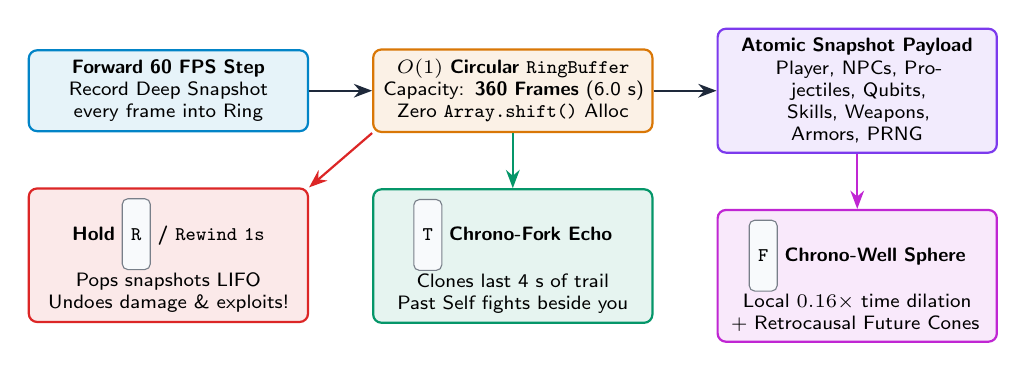
\begin{tikzpicture}[
  font=\scriptsize\sffamily,
  >=Stealth,
  blk/.style={draw=#1, fill=#1!10, rounded corners=3pt, thick, minimum height=9mm, text width=33mm, align=center, inner sep=3.5pt}
]
  \node[blk=plnCyan]    (fwd)  {\textbf{Forward 60~FPS Step}\\Record Deep Snapshot\\every frame into Ring};
  \node[blk=plnGold, right=8mm of fwd] (ring) {\textbf{$O(1)$ Circular \texttt{RingBuffer}}\\Capacity: \textbf{360 Frames} (6.0~s)\\Zero \texttt{Array.shift()} Alloc};
  \node[blk=plnViolet, right=8mm of ring] (snap) {\textbf{Atomic Snapshot Payload}\\Player, NPCs, Projectiles, Qubits,\\Skills, Weapons, Armors, PRNG};
  \node[blk=plnCrimson, below=7mm of fwd] (rew) {\textbf{Hold \kbd{R} / \texttt{Rewind 1s}}\\Pops snapshots LIFO\\Undoes damage \& exploits!};
  \node[blk=plnEmerald, below=7mm of ring] (fork) {\textbf{\kbd{T} Chrono-Fork Echo}\\Clones last 4~s of trail\\Past Self fights beside you};
  \node[blk=plnMagenta, below=7mm of snap] (well) {\textbf{\kbd{F} Chrono-Well Sphere}\\Local $0.16\times$ time dilation\\+ Retrocausal Future Cones};

  \draw[->, thick, plnSlate] (fwd) -- (ring);
  \draw[->, thick, plnSlate] (ring) -- (snap);
  \draw[->, thick, plnCrimson] (ring.south west) -- (rew.north east);
  \draw[->, thick, plnEmerald] (ring.south) -- (fork.north);
  \draw[->, thick, plnMagenta] (snap.south) -- (well.north);
\end{tikzpicture}
\caption[Temporal Causality Architecture (360-Frame RingBuffer, Echoes \& Chrono-Wells)]{Temporal Causality Architecture (\texttt{src/quantum/temporal.js}): lossless 360-frame $O(1)$ ring-buffer rewind, Chrono-Fork Past-Self Echoes, and local spherical Chrono-Wells.}
\label{fig:temporal-arch}
\end{figure}

\begin{table}[ht]
\centering
\caption{The Six Procedural Scale Realms Spanning 24 Orders of Magnitude ($10^{-15}\,\text{m} \to 10^9\,\text{m}$).}
\label{tab:realms}
\footnotesize
\begin{tabularx}{\textwidth}{@{} c L{1.4cm} L{3.3cm} c c c L{2.4cm} Y @{}}
\toprule
\textbf{\#} & \textbf{Scale} & \textbf{Realm Name} & \textbf{WKB} & \textbf{Pillars} & \textbf{Rings} & \textbf{Musical Mode} & \textbf{Realm Theme} \\
\midrule
0 & $10^{-15}$~m & \textbf{Planck Foam Crucible} & $1.45\times$ & 8 & 3 & A2 Phrygian (110~Hz) & Sub-nuclear vacuum fluctuations \& high tunneling \\
1 & $10^{-10}$~m & \textbf{Bravais Crystal Lattice} & $1.15\times$ & 12 & 2 & C3 Lydian (130.8~Hz) & Atomic diffraction ridges \& standing interference \\
2 & $10^{-3}$~m & \textbf{Planarian Cellular Nexus} & $1.00\times$ & 10 & 4 & G2 Dorian (98.0~Hz) & Living \texttt{.hbin} vascular matrix \& mitosis fields \\
3 & $10^{0}$~m & \textbf{Chronomancer Observatory} & $1.10\times$ & 6 & 5 & D3 Harm.\ Minor (146.8~Hz) & Astrolabe time-dilation rings \& retrocausal cones \\
4 & $10^{4}$~m & \textbf{Dyson Hologram Megastructure} & $1.25\times$ & 14 & 4 & E2 Whole-Tone (82.4~Hz) & Orbital monolith depths \& Bell conduit spans \\
5 & $10^{9}$~m & \textbf{Singularity Event Horizon} & $1.60\times$ & 9 & 6 & D2 Locrian (73.4~Hz) & Gravitational phase-shift \& timeline convergence \\
\bottomrule
\end{tabularx}
\end{table}

\FloatBarrier
% ============================================================================
% SECTION 5: TELEMETRY STRIP & ALL 5 WORKBENCH TABS
% ============================================================================
\section{Zones E \& F --- Live Telemetry Strip \& All 5 Workbench Tabs}
\label{sec:workbench}

\subsection{Zone E --- The 6-Box Live Telemetry Strip}
Immediately below the sliders sits a 6-tile live telemetry bar merging byte-level \texttt{.hbin} forensics with real-time quantum and combat state:
\begin{enumerate}[leftmargin=1.5em, itemsep=1.5pt]
  \item \textbf{\texttt{.hbin 3D Cells} (\texttt{0..192 / 192}):} Count of authentic Merkle-verified cells currently recovered. Green at $\ge 96$ cells, amber while degraded but bootable, crimson at \texttt{CELL DEATH}.
  \item \textbf{\texttt{RS(254,238) Healed} (\texttt{N B}):} Exact number of corrupted bytes repaired mathematically by inner 2-way interleaved Reed--Solomon decoding on the most recent decode pass (reaches \texttt{3,072 B} under a file-wide 16~B burst!).
  \item \textbf{\texttt{Byzantine Blocked} (\texttt{N}):} Number of adversarially forged RS-valid Trojan cells caught and quarantined by Depth-8 SHA-256 Merkle proofs prior to Cauchy inversion.
  \item \textbf{\texttt{Xenografts} (\texttt{N}):} Number of foreign-species organ bundles currently grafted into the living host organism.
  \item \textbf{\texttt{Q-Entropy H($\psi$)} (\texttt{0.00..4.00 b}):} Live computational-basis Shannon entropy of the 4-qubit statevector in bits.
  \item \textbf{\texttt{Decode / Hostiles} (\texttt{X.Xms $\cdot$ N NPC}):} Wall-clock decode latency of the last \texttt{.hbin} mutation in milliseconds alongside live hostile NPC count.
\end{enumerate}

\subsection{Tab 1 --- 1/1 Arsenal, Armor, Adaptive NPCs \& 12-Skill Tree}
\label{sec:tab1}

Tab~1 exposes PLANARIA's deterministic 128-bit SHA-256 \texttt{sfc32} procedural universe forge (\path{src/world/generator.js}). Every weapon, armor, NPC, and stage receives a unique 64-bit hexadecimal \textbf{Lineage Genome ID} (\nolinkurl{#XXXX-XXXX-XXXX-XXXX}). Verified by generator reachability tests (\texttt{Suite 15}) and cross-checked arithmetically in Lean~4 (\nolinkurl{combinatorial_1of1_space_exceeds_6_trillion}), the exact reachable discrete cross-product is:
\begin{equation}
  \underbrace{(14\times 10\times 12\times 8\times 6)}_{80{,}640\text{ Weapons}}
  \;\times\;
  \underbrace{(8\times 8\times 8\times 6)}_{3{,}072\text{ Armors}}
  \;\times\;
  \underbrace{((7\times 6 + 3)\times 8\times 6\times 12)}_{25{,}920\text{ Reachable NPCs}}
  \;=\;
  \mathbf{6{,}421{,}059{,}993{,}600}\; (>6.42\times 10^{12}),
\end{equation}
multiplied further by continuous stat gradients and $2^{64}$ cryptographic lineage IDs.

\begin{itemize}[leftmargin=1.5em, itemsep=1.5pt]
  \item \textbf{Top Action Buttons:} \textbf{\texttt{Forge New 1/1 Weapon \& Armor (C)}} mints a guaranteed \texttt{ENTANGLED}+ rarity weapon and armor immediately; \textbf{\texttt{Entangle Weapons \#1 $\leftrightarrow$ \#2}} prepares a real Bell state on qubits $(0,1)$ and Bell-links Weapon slots \texttt{[1]} and \texttt{[2]} so their quantum effects synchronize!
  \item \textbf{6 Rarity Tiers (Multiplier / Color):} \texttt{COHERENT} ($1.00\times$, slate), \texttt{RESONANT} ($1.28\times$, cyan), \texttt{ENTANGLED} ($1.62\times$, emerald), \texttt{CHRONO-MYTH} ($2.08\times$, violet), \texttt{SINGULARITY} ($2.72\times$, gold), and \texttt{1/1 ANOMALY} ($3.65\times$, magenta --- Slot~\texttt{[4]} starts with a guaranteed \texttt{1/1 ANOMALY} showcase weapon!).
\end{itemize}

\begin{table}[ht]
\centering
\caption{Complete 1/1 Procedural Forge Component Matrix (Weapons, Armors, NPCs \& Adaptive AI).}
\label{tab:forge-matrix}
\scriptsize
\begin{tabularx}{\textwidth}{@{} L{2.8cm} c Y @{}}
\toprule
\textbf{Category} & \textbf{\#} & \textbf{Complete Catalog of Live In-Engine Variants} \\
\midrule
\textbf{Weapon Prefixes} & 14 & Hilbert, Tachyon, Planarian, Non-Local, Eigenstate, Decoherent, Causal, Bell-Broken, Superposed, Tunneler, Chirality, Anastomotic, Zero-Cliff, Adelic. \\
\textbf{Weapon Frames} & 10 & Boson Rail-Lance (\texttt{BEAM}), Phase-Collapsed Glaive (\texttt{ARC}), Entangler Prism (\texttt{CHAIN}), Tachyon Chakram (\texttt{ORBIT}), Wavefunction Mortar (\texttt{WAVE}), Chrono-Reversal Scythe (\texttt{BOOMER}), Singularity Longbow (\texttt{PIERCE}), Hadamard Twin-Blades (\texttt{SPLIT}), Zeno Observer Carbine (\texttt{LOCK}), Hologram Splice-Cannon (\texttt{SCATTER}). \\
\textbf{Quantum Weapon Mods} & 12 & \texttt{ENTANGLE} (Bell non-local echo), \texttt{TUNNEL} (WKB pillar bypass), \texttt{SUPERPOSE} (Hadamard twin fork), \texttt{ZENO} ($-68\%$ target motion), \texttt{INTERFERENCE} ($2.2\times$ ridge crit), \texttt{COLLAPSE} (entropy implosion), \texttt{DECOHERE} (shield strip), \texttt{CAUCHY} (hit heals shield), \texttt{GHZ\_CASCADE} (3-body chain), \texttt{PHASE\_SHIFT} (Berry homing), \texttt{TUNNEL\_CRIT} ($+80\%$ post-pillar burst), \texttt{SPIN\_FLIP} (reflects enemy bullets). \\
\textbf{Temporal Weapon Mods} & 8 & \texttt{Chrono-Slow} ($0.28\times$ slow bubble), \texttt{Hyper-Clock} ($+35\%$ cadence), \texttt{Retrocausal} (auto-leads motion), \texttt{Timeline-Echo} (ghost re-fire $+0.35\text{s}$), \texttt{Entropy-Rewind} ($+4$ Chrono/hit), \texttt{Paradox-Rift} (bonus near Echo), \texttt{Zero-Tick} ($0.6\text{s}$ stasis on crit), \texttt{Self-Splitting} (mid-flight projectile mitosis). \\
\textbf{Armor Chassis} & 8 & Holographic Carapace, Cauchy-Matrix Aegis, Phase-Shift Mantle, Planarian Exoshell, Bravais Spin-Lattice, Heisenberg Cloud-Shroud, Chrono-Fold Harness, Singularity Corona. \\
\textbf{Armor Barrier Layers} & 8 & \texttt{RS(254,238) Self-Repair} ($+5$/s shield), \texttt{WKB Phase-Tunneling} ($+22\%$ dodge), \texttt{Bell-State Reflection} (45\% reflect), \texttt{Retrocausal Hit-Rewind} (auto-undo 1 lethal hit/10s), \texttt{Zeno Proximity Dampener} ($-38\%$ enemy bullet speed), \texttt{Merkle Byzantine Barrier} (full radiation decoherence immunity + 30\% boss resist), \texttt{Superposition Decoy}, \texttt{Chronon Capacitor} ($+45\%$ Chrono regen). \\
\textbf{NPC Archetypes} & 8 & Phase Weaver (\texttt{OCTA}), Tunnel Stalker (\texttt{PYRAMID}), Chronophage (\texttt{TORUS}), Bell Sentinel (\texttt{CUBE}), Interferon Prism (\texttt{DIAMOND}), Decoherence Wraith (\texttt{SPIKE}), Planarian Splitter (\texttt{ICO}), and \textbf{$\star$ BOSS: Singularity Archon} (\texttt{BOSS}). \\
\textbf{NPC Mutations} & 8 & \texttt{SUPERPOSED} (twin clones), \texttt{ENTANGLED} (Bell pair), \texttt{ZENO\_LOCKED} (freezes in gaze / hyper-blinks away), \texttt{TUNNELER} (ambushes through pillars), \texttt{INTERFERING}, \texttt{MITOTIC} (splits into 2 halves at 50\% HP!), \texttt{BYZANTINE} (drains coherence), \texttt{RESONANT}. \\
\textbf{NPC Temporal Affixes} & 6 & \texttt{SYNCED}, \texttt{DILATED\_AURA} (slow aura), \texttt{HASTENED} ($1.38\times$ speed), \texttt{RETROCAUSAL} (dodges predicted shots), \texttt{ECHOING} (afterimage mines), \texttt{REVERSING} (rewinds 1.5s of its own HP if not bursted down). \\
\textbf{Adaptive AI Counters} & 4 & Tracks your playstyle EMA (\texttt{playerProfile}): spawns \texttt{ANTI-BEAM} (if beam ratio $>0.6$), \texttt{ANTI-CLOSE} (if close kills $>0.5$), \texttt{ANTI-BELL} (if entangles $>5$), or \texttt{BASE}. \\
\bottomrule
\end{tabularx}
\end{table}

\begin{table}[ht]
\centering
\caption[All 12 Nodes of the 4-Branch Adaptive Skill Tree]{All 12 Upgradeable Nodes of the 4-Branch Adaptive Skill Tree (Max \texttt{Lv.5} Each; Click Any Card to Spend SP).}
\label{tab:skills}
\footnotesize
\begin{tabularx}{\textwidth}{@{} L{3.1cm} L{3.6cm} Y @{}}
\toprule
\textbf{Branch} & \textbf{Skill Name} & \textbf{Effect Per Rank (Levels 1--5)} \\
\midrule
\textbf{\color{plnCyan}SUPERPOSITION} & Hadamard Bifurcation & $+15\%$ damage \& wider wave-clone phase interference per rank. \\
\textbf{\color{plnCyan}SUPERPOSITION} & WKB Resonance Mastery & $+12\%$ barrier tunneling probability \& $+18\%$ post-tunnel crit damage. \\
\textbf{\color{plnCyan}SUPERPOSITION} & Squeezed-State Mastery & Boosts Heisenberg Stance crit multiplier \& probabilistic dodge ceiling. \\
\midrule
\textbf{\color{plnMagenta}ENTANGLEMENT} & Tsirelson Bell Link & Increases Bell-entangled non-local damage echo from 55\% up to 115\%. \\
\textbf{\color{plnMagenta}ENTANGLEMENT} & GHZ Multi-Body Web & Chains $+1$ additional hostile into your GHZ entanglement web every 2 ranks. \\
\textbf{\color{plnMagenta}ENTANGLEMENT} & Quantum Zeno Gaze & Direct camera sightline slows observed NPCs by up to 80\%. \\
\midrule
\textbf{\color{plnGold}CHRONOMANCY} & Chrono-Well Radius & $+20\%$ time-dilation sphere radius \& deeper localized slow-motion. \\
\textbf{\color{plnGold}CHRONOMANCY} & Paradox Echo Arsenal & Past-Timeline Echo Clones deal $+25\%$ damage \& remain active longer. \\
\textbf{\color{plnGold}CHRONOMANCY} & Zero-Drift Scrubbing & $-18\%$ Chrono Energy drain during Rewind and Bullet-Time. \\
\midrule
\textbf{\color{plnEmerald}HOLOGRAPHIC} & RS(254,238) Autophagy & $+3.5$/s shield regeneration \& rapid Werner coherence recovery. \\
\textbf{\color{plnEmerald}HOLOGRAPHIC} & Binary Mitosis Surge & Bisecting or forging emits a healing shockwave across the 3D arena. \\
\textbf{\color{plnEmerald}HOLOGRAPHIC} & Chimeric Overclock & $+22\%$ to ALL stats whenever a Cross-Species Xenograft is active! \\
\bottomrule
\end{tabularx}
\end{table}

\subsection{Tab 2 --- Dual-Patient 2D \texttt{PVM-32} \& Linear Control Twin (\texttt{LINBIN01})}
\label{sec:tab2}

Tab~2 provides a real-time scientific A/B comparison on two genuine $160\times 120$ RGBA32 phosphor displays:
\begin{itemize}[leftmargin=1.5em, itemsep=1.5pt]
  \item \textbf{Normal / Surgery Mode:} Left monitor (\texttt{PATIENT A $\cdot$ PLANARIA}) runs the real \texttt{.hbin} organism on \texttt{vmPrimary} (showing its 128-bit Lineage Root, exact instructions/frame, and \texttt{traps:0}). Right monitor (\texttt{CONTROL $\cdot$ LINEAR BINARY (LINBIN01)}) runs the exact same compiled program inside a traditional headered ELF-style executable with SHA-256 footer on \texttt{vmSecondary} receiving the \textbf{identical physical damage}. Watch the right screen flatline instantly (\texttt{LINEAR SIGSEGV}) on a single unaligned shift, 2~B radiation burst, or 15\% shred while Patient~A keeps running!
  \item \textbf{Mitosis Mode (after clicking \texttt{Laser Bisect (50/50)}):} The two monitors transform into \textbf{\texttt{MITOSIS CHILD A $\cdot$ LEFT 50\% (0..49176)}} and \textbf{\texttt{MITOSIS CHILD B $\cdot$ RIGHT 50\% (49177..98303)}} --- two completely disjoint byte files with \textbf{zero overlapping bytes}, BOTH booting simultaneously at Stratum~3 and reporting \texttt{100\% REGEN READY}!
\end{itemize}

\subsection{Tab 3 --- 192-Cell Holographic Tissue Surgery Map \& Cell Inspector}
\label{sec:tab3}

A pristine \texttt{.hbin} file is \textbf{exactly 98,304 bytes = 192 fixed 512-byte cells} with zero padding bytes wasted ($4 + 16 + 332 + 128 + 32 = 512$~B exact; Figure~\ref{fig:cell-anatomy}). Rather than laying bundles out sequentially (which would break 50/50 mitosis), PLANARIA assigns cell $i$ of bundle $b$ the exact integer numerator
\begin{equation}
  \mathrm{posNum}(b, i, n_b) = (14i + 2b + 1)\cdot\frac{480}{n_b} \in (0, 6720),
\end{equation}
sorted by pairwise-distinct integer key $\mathrm{posNum}\cdot 8 + b$ so that slots \texttt{0..95} and slots \texttt{96..191} each contain exactly $n_b/2 \ge k_b + 2$ cells of every single bundle (machine-checked in \texttt{planaria\_schedule\_nodup\_and\_sorted\_halves}).

\begin{figure}[ht]
\centering
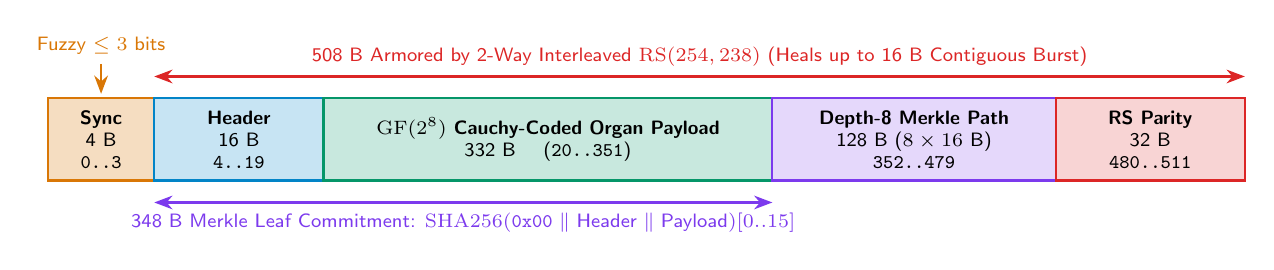
\begin{tikzpicture}[font=\scriptsize\sffamily, >=Stealth]
  \fill[plnGold!25, draw=plnGold, thick] (0,0) rectangle (1.35,1.05);
  \node[align=center] at (0.675,0.52) {\textbf{Sync}\\4~B\\\texttt{0..3}};

  \fill[plnCyan!22, draw=plnCyan, thick] (1.35,0) rectangle (3.5,1.05);
  \node[align=center] at (2.425,0.52) {\textbf{Header}\\16~B\\\texttt{4..19}};

  \fill[plnEmerald!22, draw=plnEmerald, thick] (3.5,0) rectangle (9.2,1.05);
  \node[align=center] at (6.35,0.52) {\textbf{$\mathrm{GF}(2^8)$ Cauchy-Coded Organ Payload}\\332~B \quad (\texttt{20..351})};

  \fill[plnViolet!20, draw=plnViolet, thick] (9.2,0) rectangle (12.8,1.05);
  \node[align=center] at (11.0,0.52) {\textbf{Depth-8 Merkle Path}\\128~B ($8\times 16$~B)\\\texttt{352..479}};

  \fill[plnCrimson!20, draw=plnCrimson, thick] (12.8,0) rectangle (15.2,1.05);
  \node[align=center] at (14.0,0.52) {\textbf{RS Parity}\\32~B\\\texttt{480..511}};

  \draw[thick, plnViolet, <->] (1.35,-0.28) -- (9.2,-0.28)
    node[midway, below, text=plnViolet] {348~B Merkle Leaf Commitment: $\mathrm{SHA256}(\texttt{0x00}\parallel\text{Header}\parallel\text{Payload})[0..15]$};

  \draw[thick, plnCrimson, <->] (1.35,1.32) -- (15.2,1.32)
    node[midway, above, text=plnCrimson] {508~B Armored by 2-Way Interleaved $\mathrm{RS}(254,238)$ (Heals up to 16~B Contiguous Burst)};

  \draw[thick, plnGold, ->] (0.675,1.48) -- (0.675,1.10);
  \node[above, text=plnGold] at (0.675,1.48) {Fuzzy $\le 3$~bits};
\end{tikzpicture}
\caption{Byte-exact anatomy of every 512-byte Holographic Cell displayed in the Tab~3 Cell Inspector.}
\label{fig:cell-anatomy}
\end{figure}

\begin{itemize}[leftmargin=1.5em, itemsep=1.5pt]
  \item \textbf{Color Key on the 24$\times$8 Grid:} \pill{plnGold}{Gold} = S0 Stem (\texttt{B0}, $k=2$) $\cdot$ \pill{plnCyan}{Cyan} = S1 Vital (\texttt{B1/B2}, $k=4$) $\cdot$ \pill{plnEmerald}{Emerald} = S2 Cortex (\texttt{B3/B4}, $k=6\text{--}8$) $\cdot$ \pill{plnViolet}{Purple} = S3 FX/Genome (\texttt{B5/B6}, $k=8\text{--}16$) $\cdot$ \pill{plnCrimson}{Red} = Quarantined/Necrotic $\cdot$ \pill{plnMagenta}{Magenta} = Xenografted foreign cell.
  \item \textbf{Live Manual Surgery:} Click any square (or focus canvas + \kbd{$\leftarrow$}\kbd{$\rightarrow$}\kbd{$\uparrow$}\kbd{$\downarrow$}) to view its exact byte offset, sync word bit errors, \texttt{RS(254,238)} repair count, bundle/organ, Cauchy evaluation coordinate $x_i$, $k/n$, 16-bit ABI signature, implied Merkle root, and payload hex. Hold \kbd{Shift+Drag} (or press \kbd{Delete}/\kbd{Backspace}) to carve custom surgical lesions live!
\end{itemize}

\subsection{Tab 4 --- Organ Vascular Anastomosis Graph \& Live \texttt{PVM-32} Disassembler}
\label{sec:tab4}

Tab~4 visualizes the 7 bundles (Table~\ref{tab:bundles}) and shows in real time how \texttt{PVM-32}'s hardware \texttt{ORGAN\_CALL rd, organId, maxStratum} instruction scans loaded authentic/xenografted bundles in \textbf{strictly descending stratum order} (\texttt{S3 $\to$ S2 $\to$ S1 $\to$ S0}). If a nested organ traps, \texttt{PVM-32}'s \textbf{pre-allocated zero-allocation LIFO undo journal} atomically rolls back any partial RAM or audio voice mutations and returns \texttt{0} cleanly so the Stem Nucleus invokes its emergency fallback without crashing (Figure~\ref{fig:anastomosis}). Use the \textbf{\texttt{Select Bundle to Disassemble}} dropdown to inspect live 32-bit RISC assembly (\texttt{B0..B5}) or the self-describing Genome JSON (\texttt{B6}, strictly non-executable).

\begin{table}[ht]
\centering
\caption{The Seven Progressive Holographic Bundles (\texttt{B0..B6}) and Shared-Memory ABI (\texttt{MEM[0..511]}).}
\label{tab:bundles}
\footnotesize
\begin{tabularx}{\textwidth}{@{} c L{3.1cm} L{1.7cm} c c r r r c Y @{}}
\toprule
\textbf{ID} & \textbf{Bundle Name} & \textbf{Organ} & \textbf{Str.} & \textbf{ABI} & $k_b$ & $n_b$ & \textbf{Max B} & \textbf{Tol.} & \textbf{Sovereignty} \\
\midrule
B0 & \texttt{S0\_STEM\_NUCLEUS}   & \texttt{KERNEL}   & S0 & \texttt{0x0101} &  2 & 24 &   664 & \textbf{91.7\%} & \textbf{Sovereign} (immutable) \\
B1 & \texttt{S1\_CORE\_LOGIC}     & \texttt{LOGIC}    & S1 & \texttt{0x0201} &  4 & 24 & 1,328 & 83.3\% & Xenograftable \\
B2 & \texttt{S1\_WIREFRAME}       & \texttt{RENDERER} & S1 & \texttt{0x0301} &  4 & 24 & 1,328 & 83.3\% & Xenograftable \\
B3 & \texttt{S2\_CORTEX\_RENDER}  & \texttt{RENDERER} & S2 & \texttt{0x0302} &  8 & 32 & 2,656 & 75.0\% & Xenograftable \\
B4 & \texttt{S2\_SYNTH\_AUDIO}    & \texttt{AUDIO}    & S2 & \texttt{0x0402} &  6 & 24 & 1,992 & 75.0\% & Xenograftable \\
B5 & \texttt{S3\_ORGANISM\_FX}    & \texttt{FX}       & S3 & \texttt{0x0503} & 16 & 40 & 5,312 & 60.0\% & Xenograftable \\
B6 & \texttt{S3\_GENOME\_LEDGER}  & \texttt{GENOME}   & S3 & \texttt{0x0603} &  8 & 24 & 2,656 & 66.7\% & \textbf{Sovereign} (non-exec JSON) \\
\midrule
\multicolumn{10}{@{}p{\textwidth}@{}}{\textbf{Shared-Memory World-State ABI:} \texttt{MEM[0..15]} = frame, score, energy, focal $(x,y)$, angle, combo, events, audio root/tempo, entropy, entity count, input, init, \texttt{SPECIES\_MAGIC}; \texttt{MEM[64..255]} = 24 entities $\times$ 8 words; \texttt{MEM[256..511]} = 32 particles/scope.} \\
\bottomrule
\end{tabularx}
\end{table}

\begin{figure}[ht]
\centering
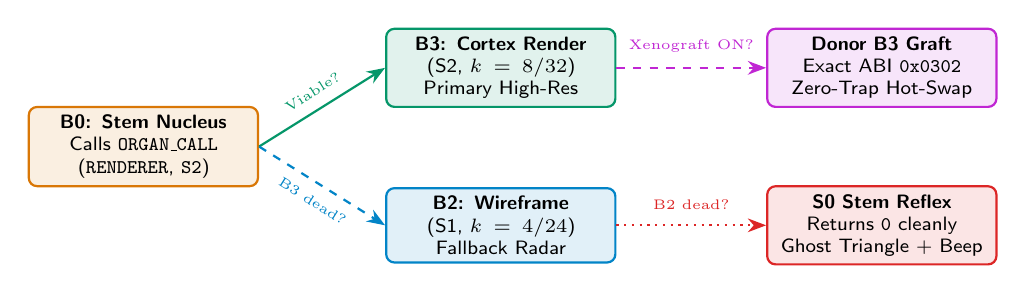
\begin{tikzpicture}[
  font=\scriptsize\sffamily,
  >=Stealth,
  nd/.style={draw=#1, fill=#1!12, rounded corners=3pt, thick, minimum height=8.5mm, text width=27mm, align=center, inner sep=3pt}
]
  \node[nd=plnGold]    (stem) {\textbf{B0: Stem Nucleus}\\Calls \texttt{ORGAN\_CALL}\\(\texttt{RENDERER}, \texttt{S2})};
  \node[nd=plnEmerald, right=16mm of stem, yshift=10mm]  (b3) {\textbf{B3: Cortex Render}\\(S2, $k=8/32$)\\Primary High-Res};
  \node[nd=plnCyan, right=16mm of stem, yshift=-10mm]    (b2) {\textbf{B2: Wireframe}\\(S1, $k=4/24$)\\Fallback Radar};
  \node[nd=plnCrimson, right=19mm of b2]               (ref) {\textbf{S0 Stem Reflex}\\Returns \texttt{0} cleanly\\Ghost Triangle + Beep};
  \node[nd=plnMagenta, right=19mm of b3]               (xeno) {\textbf{Donor B3 Graft}\\Exact ABI \texttt{0x0302}\\Zero-Trap Hot-Swap};

  \draw[->, thick, plnEmerald] (stem.east) -- node[above=1pt, sloped, font=\tiny]{Viable?} (b3.west);
  \draw[->, thick, plnCyan, dashed] (stem.east) -- node[below=1pt, sloped, font=\tiny]{B3 dead?} (b2.west);
  \draw[->, thick, plnCrimson, dotted] (b2.east) -- node[above=2pt, font=\tiny]{B2 dead?} (ref.west);
  \draw[->, thick, plnMagenta, dashed] (b3.east) -- node[above=2pt, font=\tiny]{Xenograft ON?} (xeno.west);
\end{tikzpicture}
\caption[Hardware \texttt{ORGAN\_CALL} Control-Flow Anastomosis Graph]{Hardware \texttt{ORGAN\_CALL} Control-Flow Anastomosis routing shown live in Tab~4.}
\label{fig:anastomosis}
\end{figure}

\subsection{Tab 5 --- Empirical Survival Curve \& Live In-Browser \texttt{Plang} Compiler}
\label{sec:tab5}

\begin{itemize}[leftmargin=1.5em, itemsep=1.5pt]
  \item \textbf{Top Chart (Empirical Phase-Transition Curve):} Renders the pre-registered paired 4-architecture Monte Carlo data from \texttt{results/benchmarks.json} ($N = 40$ paired seeds $\times$ 25 erasure points = 4,000 evaluations; Figure~\ref{fig:survival-curve}) with a live vertical cursor tracking your current \texttt{.hbin} binary's erasure level.
  \item \textbf{Bottom Live \texttt{Plang} Compiler Editor:} Displays the complete live source code of the active species. Edit constants, gameplay speeds, colors, synth frequencies, or bundle instructions directly inside the browser and click \textbf{\texttt{Compile \& Inject Live .hbin}} to run the full \texttt{Plang $\to$ PVM-32 $\to$ Cauchy $\to$ Merkle $\to$ RS(254,238)} build pipeline in $\sim 12$~ms and hot-inject your brand-new 96~KiB living binary straight into the running engine!
\end{itemize}

\begin{figure}[ht]
\centering
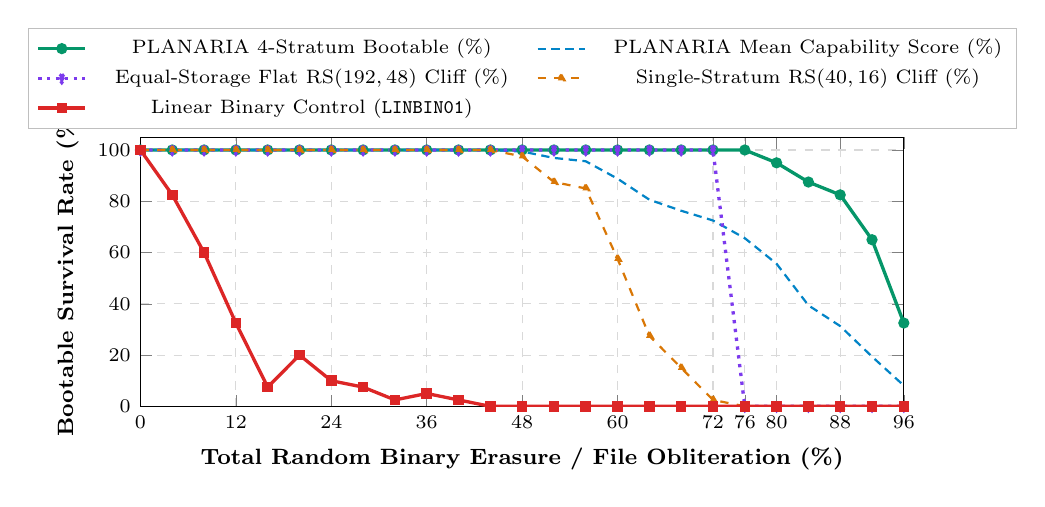
\begin{tikzpicture}
\begin{axis}[
  width=0.93\textwidth,
  height=5.0cm,
  xlabel={Total Random Binary Erasure / File Obliteration (\%)},
  ylabel={Bootable Survival Rate (\%)},
  xmin=0, xmax=96,
  ymin=0, ymax=105,
  xtick={0,12,24,36,48,60,72,76,80,88,96},
  ytick={0,20,40,60,80,100},
  grid=major,
  grid style={dashed, gray!30},
  legend columns=2,
  legend style={at={(0.5,1.03)}, anchor=south, font=\scriptsize, fill=white, draw=gray!50, column sep=8pt},
  tick label style={font=\scriptsize},
  label style={font=\footnotesize\bfseries}
]
  \addplot[color=plnEmerald, very thick, mark=*, mark size=1.4pt] coordinates {
    (0,100) (4,100) (8,100) (12,100) (16,100) (20,100) (24,100) (28,100)
    (32,100) (36,100) (40,100) (44,100) (48,100) (52,100) (56,100) (60,100)
    (64,100) (68,100) (72,100) (76,100) (80,95.0) (84,87.5) (88,82.5) (92,65.0) (96,32.5)
  };
  \addlegendentry{PLANARIA 4-Stratum Bootable (\%)}

  \addplot[color=plnCyan, thick, densely dashed] coordinates {
    (0,100) (4,100) (8,100) (12,100) (16,100) (20,100) (24,100) (28,100)
    (32,100) (36,100) (40,100) (44,100) (48,99.4) (52,96.9) (56,95.6) (60,88.8)
    (64,80.6) (68,76.3) (72,72.5) (76,65.6) (80,55.6) (84,39.4) (88,31.3) (92,19.4) (96,8.1)
  };
  \addlegendentry{PLANARIA Mean Capability Score (\%)}

  \addplot[color=plnViolet, very thick, dotted, mark=diamond*, mark size=1.5pt] coordinates {
    (0,100) (4,100) (8,100) (12,100) (16,100) (20,100) (24,100) (28,100)
    (32,100) (36,100) (40,100) (44,100) (48,100) (52,100) (56,100) (60,100)
    (64,100) (68,100) (72,100) (76,0) (80,0) (84,0) (88,0) (92,0) (96,0)
  };
  \addlegendentry{Equal-Storage Flat $\mathrm{RS}(192,48)$ Cliff (\%)}

  \addplot[color=plnGold, thick, dashed, mark=triangle*, mark size=1.4pt] coordinates {
    (0,100) (4,100) (8,100) (12,100) (16,100) (20,100) (24,100) (28,100)
    (32,100) (36,100) (40,100) (44,100) (48,97.5) (52,87.5) (56,85.0) (60,57.5)
    (64,27.5) (68,15.0) (72,2.5) (76,0) (80,0) (84,0) (88,0) (92,0) (96,0)
  };
  \addlegendentry{Single-Stratum $\mathrm{RS}(40,16)$ Cliff (\%)}

  \addplot[color=plnCrimson, very thick, mark=square*, mark size=1.3pt] coordinates {
    (0,100) (4,82.5) (8,60.0) (12,32.5) (16,7.5) (20,20.0) (24,10.0) (28,7.5)
    (32,2.5) (36,5.0) (40,2.5) (44,0) (48,0) (52,0) (56,0) (60,0)
    (64,0) (68,0) (72,0) (76,0) (80,0) (84,0) (88,0) (92,0) (96,0)
  };
  \addlegendentry{Linear Binary Control (\texttt{LINBIN01})}
\end{axis}
\end{tikzpicture}
\caption[Empirical 4-Architecture Survival Curve (Tab~5)]{Pre-registered paired 4-architecture empirical survival curve (\texttt{results/benchmarks.json}, plotted live in Tab~5). Equal-storage flat $\mathrm{RS}(192,48)$ collapses from 100\% to 0\% at 75\% erasure, whereas PLANARIA executes through 76--96\% erasure ($p_{\text{Holm}} \le 4.88\times 10^{-3}$).}
\label{fig:survival-curve}
\end{figure}

\FloatBarrier
% ============================================================================
% SECTION 6: RIGHT VIVISECTION DOCK & 48 KHZ AUDIOWORKLET DSP
% ============================================================================
\section{Zones G \& H --- Live \texttt{.hbin} 3D Vivisection Dock, Event Log \& Audio DSP}
\label{sec:dock}

Every single control in \textbf{Zone G (Right-Hand Dock)} executes a genuine byte-level operation on the live 98,304-byte \texttt{.hbin} buffer in RAM, applies the matching control mutation to \texttt{LINBIN01}, re-decodes both binaries immediately, hot-swaps \texttt{PVM-32} without losing RAM game state, morphs the 3D scene and audio, and appends a timestamped cryptographic audit line to \textbf{Zone H (Chrono-Quantum \& Surgical Event Log)}.

{\footnotesize
\begin{longtable}{@{} L{3.2cm} L{2.9cm} L{5.2cm} L{4.8cm} @{}}
\caption{Exhaustive Button-by-Button Reference for All 19 Controls in Zone G (Live Vivisection Dock).}
\label{tab:dock-all} \\
\toprule
\textbf{Group \& Button} & \textbf{Byte Operation} & \textbf{What PLANARIA (\texttt{.hbin}) Does} & \textbf{3D / Audio / Control Twin Effect} \\
\midrule
\endfirsthead
\toprule
\textbf{Group \& Button} & \textbf{Byte Operation} & \textbf{What PLANARIA (\texttt{.hbin}) Does} & \textbf{3D / Audio / Control Twin Effect} \\
\midrule
\endhead
\multicolumn{4}{@{}l@{}}{\textbf{\color{plnCyan}Group 1 --- Planarian Mitosis \& Regeneration}} \\*
\texttt{Laser Bisect (50/50)} & Slices pristine file at unaligned prime byte \texttt{49177} (0 shared bytes) & Decodes BOTH Left (\texttt{0..49176}) and Right (\texttt{49177..98303}) independently at S3; verifies SHA-256 bit-exact regeneration on both halves & Triggers 3D Mitosis shockwave + shield surge; Tab~2 switches to live \textbf{Child A vs.\ Child B} twin displays \\
\texttt{Regenerate 100\%} & Calls \texttt{regenerateHbin()} from surviving shards & Re-encodes all 7 bundles back into a pristine 98,304~B \texttt{.hbin} (refused if Immune is OFF or below rank $k$) & Restores all 192 orbiting 3D crystals; seals new chimera root if regenerating a Xenograft \\
\texttt{+137B Shift \& Shuffle} & Prepends 137 garbage bytes + shuffles all 192 cells & Sliding sync correlator + backward flywheel recovers every unaligned cell at S3 & PLANARIA stays 100\% alive; \texttt{LINBIN01} crashes immediately (\texttt{LINEAR SIGSEGV}) \\
\texttt{Trisect \& cat(A+C)} & Splits into 3 thirds, discards middle, concatenates \texttt{A + 97B noise + C} & Harvests surviving cells across both non-contiguous fragments; super-additively jumps back to S3 & PLANARIA heals to full 3D; \texttt{LINBIN01} flatlines \\
\midrule
\multicolumn{4}{@{}l@{}}{\textbf{\color{plnGold}Group 2 --- Progressive Erasure (3D Stratum Morph!)}} \\*
\texttt{Shred 35\% (S3 3D)} & Randomly erases 35\% of cells ($\sim 67$ cells lost) & Retains full rank across all 7 bundles $\implies$ S3 intact & Full 3D continues seamlessly; \texttt{LINBIN01} dies \\
\texttt{Shred 62\% (S2 3D)} & Randomly erases 62\% of cells & Drops S3 FX (\texttt{B5}, $k=16/40$); retains S2 Cortex + Audio & 3D morphs live to \textbf{Stratum~2 Cortex 3D}; \texttt{LINBIN01} dead \\
\texttt{Shred 78\% (S1 Wire)} & Randomly erases 78\% (past flat RS 75\% cliff!) & Drops S2 (\texttt{B3/B4}); retains S1 Logic + Wireframe (\texttt{B1/B2}) & 3D morphs live to \textbf{Stratum~1 Wireframe}; flat \texttt{RS(192,48)} \& \texttt{LINBIN01} both 0\% dead \\
\texttt{Shred 88\% (S0 Cloud)} & Randomly erases 88\% (only $\sim 23$ cells left!) & Retains $\ge 2$ cells of \texttt{B0} Stem Nucleus (91.7\% tolerance) & 3D morphs live to \textbf{Stratum~0 Ghost Point Cloud} (``The 12\% Ghost'') \\
\midrule
\multicolumn{4}{@{}l@{}}{\textbf{\color{plnCrimson}Group 3 --- Radiation Decoherence (Inner \texttt{RS(254,238)})}} \\*
\texttt{8B/Cell Random} & Corrupts 8 random bytes inside ALL 192 cells (1,536~B) & Inner interleaved RS heals 192/192 cells (100\% bit-exact) & Induces Werner decoherence on 4-qubit meter (unless Merkle Armor equipped); \texttt{LINBIN01} dead \\
\texttt{14B Burst ALL Cells} & Injects 14~B contiguous burst in ALL 192 cells (2,688~B) & Even/odd lanes each see $\le 7 \le 8$ errors $\implies$ 192/192 repaired & \texttt{RS Healed = 2,688 B}; 100\% alive; \texttt{LINBIN01} dead \\
\texttt{16B Max Burst Limit} & Injects 16~B contiguous burst in ALL 192 cells (3,072~B = 3.13\%) & Exact theoretical tight limit ($8$ errors/lane) $\implies$ 192/192 repaired! & \texttt{RS Healed = 3,072 B}; sharp boundary demo; \texttt{LINBIN01} dead \\
\texttt{22B Lethal Overdose} & Injects 22~B contiguous burst in ALL 192 cells (4,224~B) & Exceeds $t=8$ in both lanes ($11 > 8$) $\implies$ 0/192 accepted, \textbf{0 silent miscorrections} & Deliberate falsification test: clean \texttt{CELL DEATH} (click \texttt{Restore 100\%} to recover) \\
\midrule
\multicolumn{4}{@{}l@{}}{\textbf{\color{plnViolet}Group 4 --- Byzantine Trojan Immune System}} \\*
\texttt{Inject +36 Trojans} & Prepends 36 forged cells with \emph{valid zero-error RS parity} & \textbf{Immune ON:} 36/36 quarantined by Merkle proof before Cauchy decode. \textbf{Immune OFF:} poisons Gaussian elimination! & Proves live why per-cell cryptographic authentication MUST precede linear erasure decoding \\
\texttt{Immune: ON / OFF} & Toggles \texttt{disableImmuneSystem} flag & Switches between Pinned Merkle Quarantine (safe) and unprotected Cauchy decoding (deliberate attack demo) & Top badge turns crimson \texttt{IMMUNE: OFF (UNSAFE!)}; disables \texttt{Regenerate 100\%} to prevent sealing poisoned code \\
\midrule
\multicolumn{4}{@{}l@{}}{\textbf{\color{plnGold}Group 5 --- Targeted Organ Scalpel (Anastomosis)}} \\*
\texttt{Amputate S3 FX} & Excises every cell of Bundle~\texttt{B5} & Organ FX drops cleanly; \texttt{ORGAN\_CALL} returns \texttt{0} & 3D particle/FX layer disappears live with 0 traps \\
\texttt{Amputate S2 Render} & Excises every cell of Bundle~\texttt{B3} & Renderer falls back via \texttt{ORGAN\_CALL} to \texttt{B2} Wireframe & 3D \& Tab~2 step down to wireframe live; check Tab~4 graph! \\
\texttt{Amputate S2 Audio} & Excises every cell of Bundle~\texttt{B4} & Audio organ returns \texttt{0}; Stem Nucleus drops to 1-bit heartbeat & Live 48~kHz audio immediately drops rich synth to pulse \\
\texttt{Amputate All Visuals} & Excises both \texttt{B2} and \texttt{B3} & All renderer bundles gone; Stem Nucleus invokes S0 reflex & 3D/2D drops to emergency Ghost mode without crashing \\
\midrule
\multicolumn{4}{@{}l@{}}{\textbf{\color{plnMagenta}Group 6 --- Cross-Species Xenograft Chimera}} \\*
\texttt{Donor} Dropdown & Selects a second compiled species & Supplies authenticated foreign organ clusters (\texttt{B3, B4}) & Must differ from active host species \\
\texttt{Amputate \& Splice 3D Xenograft Chimera!} & Amputates host \texttt{B3/B4} + concatenates donor bytes (+53~B noise gap) & Verifies live host (\texttt{B0} viable), enforces \texttt{B0}/\texttt{B6} host sovereignty, verifies 16-bit ABI signatures, grafts foreign Render+Audio live! & Badge turns magenta \texttt{CHIMERA 3D}; 192-cell map shows magenta cells; donor audio drives host; activates \texttt{Chimeric Overclock} skill! \\
\bottomrule
\end{longtable}
}

\begin{figure}[ht]
\centering
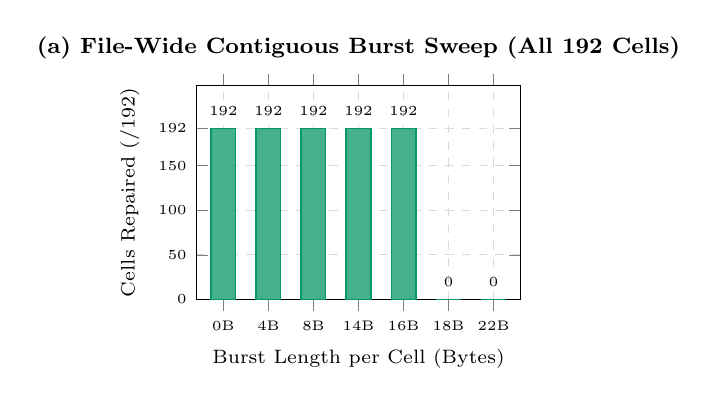
\begin{tikzpicture}
\begin{axis}[
  ybar,
  width=0.47\textwidth,
  height=4.3cm,
  title={\footnotesize\bfseries (a) File-Wide Contiguous Burst Sweep (All 192 Cells)},
  xlabel={\scriptsize Burst Length per Cell (Bytes)},
  ylabel={\scriptsize Cells Repaired (/192)},
  symbolic x coords={0B, 4B, 8B, 14B, 16B, 18B, 22B},
  xtick=data,
  ymin=0, ymax=240,
  ytick={0,50,100,150,192},
  bar width=9pt,
  grid=major,
  grid style={dashed, gray!30},
  tick label style={font=\tiny},
  nodes near coords,
  nodes near coords style={font=\tiny\bfseries, yshift=1pt}
]
  \addplot[fill=plnEmerald!75, draw=plnEmerald] coordinates {(0B,192) (4B,192) (8B,192) (14B,192) (16B,192) (18B,0) (22B,0)};
\end{axis}
\end{tikzpicture}
\hfill
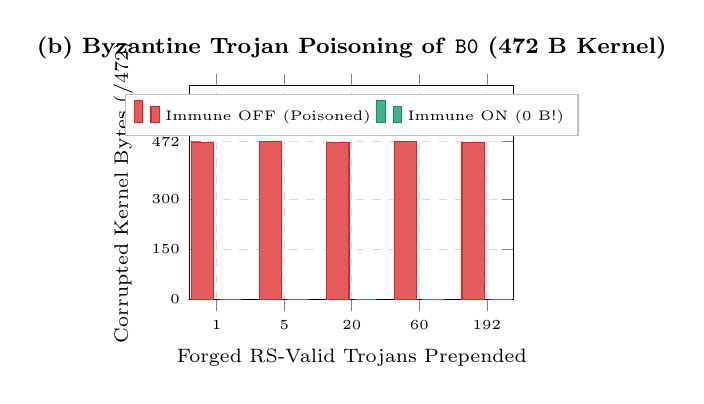
\begin{tikzpicture}
\begin{axis}[
  ybar,
  width=0.47\textwidth,
  height=4.3cm,
  title={\footnotesize\bfseries (b) Byzantine Trojan Poisoning of \texttt{B0} (472~B Kernel)},
  xlabel={\scriptsize Forged RS-Valid Trojans Prepended},
  ylabel={\scriptsize Corrupted Kernel Bytes (/472)},
  symbolic x coords={1, 5, 20, 60, 192},
  xtick=data,
  ymin=0, ymax=640,
  ytick={0,150,300,472},
  bar width=8pt,
  grid=major,
  grid style={dashed, gray!30},
  legend style={at={(0.5,0.96)}, anchor=north, font=\tiny, legend columns=2, fill=white, draw=gray!50},
  tick label style={font=\tiny}
]
  \addplot[fill=plnCrimson!75, draw=plnCrimson] coordinates {(1,469) (5,471) (20,470) (60,472) (192,470)};
  \addlegendentry{Immune OFF (Poisoned)}
  \addplot[fill=plnEmerald!75, draw=plnEmerald] coordinates {(1,0) (5,0) (20,0) (60,0) (192,0)};
  \addlegendentry{Immune ON (0~B!)}
\end{axis}
\end{tikzpicture}
\caption[Empirical Radiation Burst Knife-Edge \& Byzantine Trojan Poisoning Results]{Measured empirical knife-edge results powering Dock Groups 3 \& 4 (\texttt{results/benchmarks.json}, \texttt{v2.4.0}): (a)~192/192 cells healed up to 16~B/cell (3,072~B total), dropping sharply to 0/192 with 0 silent miscorrections at 18--22~B; (b)~even 1 RS-valid Trojan corrupts 469/472~B (99.4\%) when Merkle Immune is OFF versus 0~B when ON.}
\label{fig:rad-byz}
\end{figure}

\subsection{48~kHz Lock-Free 4-Voice PolyBLEP \texttt{AudioWorklet} DSP Chain}
\label{sec:audio}

Toggling \textbf{\texttt{48kHz Audio: ON}} starts a dedicated audio-thread worklet (\texttt{src/web/audio-worklet.js}, verified in sandboxed \texttt{Suite 29}) with zero garbage-collection allocations inside \texttt{process()}:
\begin{itemize}[leftmargin=1.5em, itemsep=1.5pt]
  \item \textbf{4 Independent Hardware Voices:} Driven by \texttt{PVM-32}'s Bundle~4 audio register bank + active Scale Realm musical mode (Table~\ref{tab:realms}), with strict finite clamping (\texttt{freqHz} $\in [20, 8000]$, \texttt{detune} $\in [-2400, +2400]$ cents, \texttt{filter} $\in [120, 14000]$~Hz).
  \item \textbf{5 Oscillator Waveforms:} \texttt{0 = OFF}, \texttt{1 = Sine}, \texttt{2 = Triangle}, \texttt{3 = PolyBLEP Anti-Aliased Sawtooth}, \texttt{4 = PolyBLEP Anti-Aliased Square}, \texttt{5 = xorshift32 White Noise}.
  \item \textbf{Click-Free Signal Chain:} Sample-rate-invariant 2.6~ms amplitude slewing $\to$ per-voice one-pole resonant lowpass filter with subnormal flush ($<10^{-15}\to 0$) $\to$ stereo panning $\to$ master soft \texttt{tanh} limiter $\to$ 20~Hz DC-blocking highpass filter.
\end{itemize}

\FloatBarrier
% ============================================================================
% SECTION 7: STEP-BY-STEP GUIDED WALKTHROUGHS & 8 LAB EXPERIMENTS
% ============================================================================
\section{Step-by-Step Guided Walkthroughs \& 8 Hands-On Lab Experiments}
\label{sec:labs}

\calloutbox{plnEmerald}{plnEmeraldBg}{WALKTHROUGH 0: YOUR FIRST 60 SECONDS IN THE LIVE GUI}{%
\begin{enumerate}[leftmargin=1.5em, itemsep=1.5pt]
  \item Open \href{https://0thernes.github.io/planaria/}{\nolinkurl{https://0thernes.github.io/planaria/}}. Wait 1~second for the 3D arena and 192 orbiting holographic cell crystals to appear.
  \item \textbf{Drag the 3D viewport} with your mouse to orbit and \textbf{scroll the wheel} to zoom in on the glowing interference floor and orbiting cells.
  \item Click \textbf{\texttt{48kHz Audio: ON}} in the top bar to hear the live 4-voice synth driven by Bundle~4.
  \item Click \textbf{\texttt{Scale 10\^{}x}} (or press \kbd{X}) a few times to watch the entire universe shift from Planck Foam ($10^{-15}$~m) through Bravais Crystal, Planarian Nexus, Chronomancer Observatory, Dyson Megastructure, to Singularity Event Horizon ($10^9$~m) --- notice the musical mode and colors transform every click!
  \item Click \textbf{\texttt{Laser Bisect (50/50)}} on the right dock, switch to \textbf{Tab~2}, and watch BOTH zero-overlap halves of the binary running live side by side. Then click \textbf{\texttt{Restore 100\%}}.
\end{enumerate}
}

\subsection{Lab 1 --- Zero-Overlap Planarian Binary Mitosis \& Bit-Exact Regeneration}
\begin{enumerate}[leftmargin=1.6em, itemsep=1.5pt]
  \item Select \texttt{AEGIS\_DRIFT.hbin} in the top dropdown and open \textbf{Tab~2} (\texttt{Dual-Patient 2D PVM-32}). Note the 16-char Lineage Root on Patient~A.
  \item On the right dock (Group~1), click \textbf{\texttt{Laser Bisect (50/50)}}. PLANARIA slices the 98,304~B binary at unaligned prime offset \texttt{49177} (zero shared bytes).
  \item Observe: BOTH monitors in Tab~2 now run independently (\texttt{Child A: 0..49176} and \texttt{Child B: 49177..98303}) at \textbf{Stratum~3}, and Zone~H logs \texttt{SHA-256 bit-exact=true}.
  \item Open \textbf{Tab~3} (\texttt{Tissue Map}) to see the sharp cyan vertical bisection line at cell~96 --- only 96 cells remain, yet every bundle still exceeds its Cauchy threshold $k_b$.
  \item Click \textbf{\texttt{Regenerate 100\%}} in Group~1. Watch \texttt{.hbin 3D Cells} jump back from \texttt{96 / 192} to \texttt{192 / 192} with the exact original SHA-256 digest!
\end{enumerate}

\subsection{Lab 2 --- ``The 12\% Ghost'': Surviving 88\% File Destruction Past the Erasure Cliff}
\begin{enumerate}[leftmargin=1.6em, itemsep=1.5pt]
  \item Click \textbf{\texttt{Restore 100\%}}, then step progressively through Dock Group~2: click \textbf{\texttt{Shred 35\%}}, \textbf{\texttt{Shred 62\%}}, \textbf{\texttt{Shred 78\%}}, and finally \textbf{\texttt{Shred 88\% (S0 Cloud)}}.
  \item Watch the 3D arena physically step down across strata: \texttt{S3 Full 3D $\to$ S2 Cortex $\to$ S1 Wireframe $\to$ S0 Ghost Cloud}.
  \item Check \textbf{Tab~2}: the classical \texttt{LINBIN01} Control Twin flatlined (\texttt{LINEAR SIGSEGV}) on the very first shred, while Patient~A continues running in Ghost survival mode with only $\sim 23$ surviving cells!
  \item Open \textbf{Tab~5} (\texttt{Survival Curve}): notice the live vertical marker at 88\% erasure sitting well past the vertical 75\% cliff where even Equal-Storage Flat $\mathrm{RS}(192,48)$ is 0.0\% dead.
\end{enumerate}

\subsection{Lab 3 --- File-Wide Contiguous Radiation Knife-Edge (16~B Heal vs.\ 22~B Overdose)}
\begin{enumerate}[leftmargin=1.6em, itemsep=1.5pt]
  \item Click \textbf{\texttt{Restore 100\%}}, then in Dock Group~3 click \textbf{\texttt{16B Max Burst Limit}}.
  \item Observe Zone~E: \texttt{RS(254,238) Healed = 3,072 B} and \texttt{.hbin 3D Cells = 192 / 192}! Every single cell in the file suffered a 16-byte contiguous burst error (zero untouched cells!), yet 100\% healed bit-exact (while \texttt{COHER} dipped from Lindblad decoherence and \texttt{LINBIN01} died).
  \item Now click \textbf{\texttt{22B Lethal Overdose}} to test Popperian falsifiability: because $11 > t = 8$ errors per RS lane, the mandatory zero-syndrome recheck rejects all 192 cells cleanly with \textbf{0 silent miscorrections} (\texttt{CELL DEATH}). Click \textbf{\texttt{Restore 100\%}}.
\end{enumerate}

\subsection{Lab 4 --- Byzantine Trojan Flood Proof (Merkle Quarantine ON vs.\ OFF)}
\begin{enumerate}[leftmargin=1.6em, itemsep=1.5pt]
  \item Ensure Group~4 shows \textbf{\texttt{Immune: ON (Safe)}}. Click \textbf{\texttt{Inject +36 Trojans}}.
  \item Observe Zone~E: \texttt{Byzantine Blocked = 36}, \texttt{.hbin 3D Cells = 192 / 192}, zero poisoning.
  \item Now click \textbf{\texttt{Immune: ON (Safe)}} to toggle it to crimson \textbf{\texttt{Immune: OFF (Unsafe!)}} and click \textbf{\texttt{Inject +36 Trojans}} again.
  \item Watch Zone~H report raw Cauchy poisoning and try clicking \textbf{\texttt{Regenerate 100\%}} --- PLANARIA refuses to re-seal untrusted poisoned memory until you re-enable Merkle Immune and restore!
\end{enumerate}

\subsection{Lab 5 --- Targeted Vascular Amputation \& Live \texttt{ORGAN\_CALL} Anastomosis}
\begin{enumerate}[leftmargin=1.6em, itemsep=1.5pt]
  \item Restore to 100\%, turn \textbf{\texttt{48kHz Audio: ON}}, and open \textbf{Tab~4} (\texttt{Organ Anastomosis \& Disasm}).
  \item In Group~5, click \textbf{\texttt{Amputate S2 Render}} and \textbf{\texttt{Amputate S2 Audio}}.
  \item Watch the Tab~4 vascular diagram dynamically reroute \texttt{RENDERER} calls from amputated \texttt{B3} down to surviving \texttt{B2} Wireframe, hear the live synth drop cleanly to Stem heartbeat, and select \texttt{B3} in the Disassembler dropdown to confirm \texttt{AMPUTATED --- Anastomosis reroutes to lower strata}.
  \item Switch to \textbf{Tab~3} and hold \kbd{Shift+Drag} across a few cells to excise individual 512-byte cells by hand!
\end{enumerate}

\subsection{Lab 6 --- Cross-Species Executable Xenograft Chimera \& \texttt{.hbin} Export}
\begin{enumerate}[leftmargin=1.6em, itemsep=1.5pt]
  \item Select \texttt{AEGIS\_DRIFT.hbin} as host, turn \textbf{\texttt{48kHz Audio: ON}}, and verify \texttt{Donor: SYNTH\_REACTOR} is selected in Group~6.
  \item In \textbf{Tab~1}, click \textbf{\texttt{Chimeric Overclock}} in the Skill Tree to spend 1 of your starting \texttt{2 SP} ($+22\%$ all stats while chimeric!).
  \item Click \textbf{\texttt{Amputate \& Splice 3D Xenograft Chimera!}} in Group~6.
  \item Observe: top badge turns magenta \textbf{\texttt{CHIMERA 3D $\cdot$ S3}}, \texttt{Xenografts = 2}, Tab~3 lights up with magenta donor cells while Host \texttt{B0}/\texttt{B6} stay strictly sovereign, and \texttt{SYNTH\_REACTOR}'s Lydian FM synth now plays live inside \texttt{AEGIS\_DRIFT}!
  \item Click \textbf{\texttt{Regenerate 100\%}} to mint a fresh standalone Chimera Lineage Root, then click \textbf{\texttt{Export .hbin}} to download your working hybrid executable.
\end{enumerate}

\subsection{Lab 7 --- Quantum-Temporal Combat Mastery}
\begin{enumerate}[leftmargin=1.6em, itemsep=1.5pt]
  \item Turn \textbf{\texttt{Autopilot: OFF}} in the top bar; fly with \kbd{W}\kbd{A}\kbd{S}\kbd{D} and shoot with \kbd{Space}.
  \item In \textbf{Tab~1}, click \textbf{\texttt{Entangle Weapons \#1 $\leftrightarrow$ \#2}}, press \kbd{4} to equip your starting \texttt{1/1 ANOMALY} weapon, then press \kbd{E} (\texttt{BELL ENTANGLE}) to tether nearby enemies in a magenta GHZ web.
  \item Slide \textbf{Heisenberg Stance} right to \texttt{90} (\texttt{MOMENTUM-BLUR}) for up to $2.45\times$ crits + 58\% dodge, press \kbd{Q} (\texttt{HADAMARD SPLIT}), press \kbd{F} (\texttt{CHRONO-WELL}) to freeze oncoming shots, and press \kbd{T} (\texttt{CHRONO-FORK ECHO}) to fight alongside your own Past Self!
  \item Take a hit, then immediately \textbf{hold \kbd{R}} (or click \textbf{\texttt{Rewind 1s}}) to watch bullets fly backwards, your HP restore, and the entire universe scrub cleanly back in time. Finish with \kbd{V} (\texttt{WAVE COLLAPSE}).
\end{enumerate}

\subsection{Lab 8 --- Live In-Browser \texttt{Plang} Coding \& Standalone CLI Round-Trip}
\begin{enumerate}[leftmargin=1.6em, itemsep=1.5pt]
  \item Open \textbf{Tab~5} and scroll down to the \texttt{Plang} source editor. Edit a constant or color in \texttt{S2\_CORTEX\_RENDER} and click \textbf{\texttt{Compile \& Inject Live .hbin}}.
  \item Check the status bar (\texttt{Compiled ... in ~12 ms -> 98,304B .hbin}) and open \textbf{Tab~2} to see your modified bytecode executing immediately inside \texttt{PVM-32}.
  \item Export the binary via \textbf{\texttt{Export .hbin}} and verify it from any terminal using the standalone CLI (Section~\ref{sec:cli}): \texttt{node bin/planaria.mjs inspect <file.hbin>}.
\end{enumerate}

\FloatBarrier
% ============================================================================
% SECTION 8: PROOF BLUEPRINT, LEAN 4.35.0 & STANDALONE CLI REFERENCE
% ============================================================================
\section{Interactive Proof Blueprint (\texttt{/blueprint/}), Lean~4.35.0 \& CLI Reference}
\label{sec:blueprint}

Clicking \textbf{\texttt{PROOF BLUEPRINT}} in the top header bar opens \href{https://0thernes.github.io/planaria/blueprint/}{\nolinkurl{https://0thernes.github.io/planaria/blueprint/}}, a dedicated zero-dependency interactive verification explorer backed by \texttt{blueprint/blueprint.json} (verified 1:1 against \texttt{lean/comparator.json} on every CI run).

\subsection{Every Element on the Proof Blueprint Page}
\begin{itemize}[leftmargin=1.5em, itemsep=1.5pt]
  \item \textbf{Top Navigation Pills:} \texttt{$\leftarrow$ 3D Vivisection Studio} (returns to main GUI), \texttt{blueprint.json} (machine-readable DAG), \texttt{lean4-audit.txt} (verbatim 85-line \texttt{\#print axioms} log, SHA-256 \texttt{13d723722ac5d5af...}), and \texttt{6-Kernel Log} (\texttt{lean4-multi-kernel.txt}).
  \item \textbf{5 KPI Cards:} Audited Theorems (\texttt{85 / 85}), Proof Modules (\texttt{7 pure modules}), Dependency Edges (\texttt{18 intra-proof}), Kernel Checks (\texttt{6 (Comparator Paranoid)}; Lean default \& paranoid share the Lean C++ kernel), and Forbidden Axioms (\texttt{0 (sorryAx / native)}).
  \item \textbf{Interactive SVG Dependency Graph (Left Card):} 7 color-coded columns (one per Lean module) displaying all 85 theorems as clickable nodes wired with curved cyan dependency edges.
  \item \textbf{Theorem Inspector (Right Card):} Clicking any DAG node or table row displays its fully qualified name, exact axiom pill (four-way breakdown: \textbf{15 axiom-free}, \textbf{12 \texttt{[propext]} only}, \textbf{40 \texttt{[propext, Quot.sound]}}, and \textbf{18 \texttt{[propext, Classical.choice, Quot.sound]}}), linked \texttt{CLAIMS.md} badges (\texttt{C01..C10}), docstring, exact \texttt{file:Lstart-Lend} source location, verbatim Lean~4.35.0 type signature, and both \texttt{Uses} and \texttt{Used by} dependency lists.
  \item \textbf{Searchable \& Filterable Master Table (Bottom Card):} Type any keyword or Claim ID (e.g., \texttt{C04}, \texttt{merkle}, \texttt{Cauchy}, \texttt{refute}) or choose one of the 7 modules from the dropdown to filter all 85 theorems live.
\end{itemize}

\begin{table}[ht]
\centering
\caption[The 7 Pure Lean~4.35.0 Proof Modules (6 Kernel Checks)]{The 7 Pure Lean~4.35.0 Proof Modules (\texttt{autoImplicit=false}, Zero Mathlib, 6 Kernel Checks; see \texttt{ERRATA.md} for scope notes).}
\label{tab:lean-modules}
\footnotesize
\begin{tabularx}{\textwidth}{@{} c L{3.6cm} c Y @{}}
\toprule
\textbf{\#} & \textbf{Lean Module} & \textbf{Thms} & \textbf{Verified Mathematical \& Protocol Model Guarantees} \\
\midrule
I & \texttt{GF256.lean} & 16 & Full 65,536-pair commutativity, 16.7M-triple associativity, all 255 inverses, \texttt{gf256Field}, universal $2\times 2$ Cauchy decode + witness. \\
II & \texttt{MitosisBounds.lean} & 14 & Tight iff mitosis placement bounds ($N\ge 2k$ / $N<2k$) + 2 witnesses, unaligned cut ($N\ge 2k+2$), \texttt{all192LexKeys.Nodup} + sorted halves, 512~B/98,304~B budgets. \\
III & \texttt{StratumAnastomosis.lean} & 8 & 7-bundle viability matching \texttt{hbin.js} Step~4 bit-for-bit, zero-crash 6-organ \texttt{resolveOrgan}, monotonicity + witness, definitional separation illustration vs.\ flat cliffs. \\
IV & \texttt{ByzantineImmune.lean} & 18 & Byte-list Hamming triangle inequality, Singleton-bound radius arithmetic + unique-decoding ball, tight 16/17/18~B burst-to-lane counts, dual-path Merkle binding, filter quarantine (under \texttt{HashBinding}), quorum majority, tie fail-closed \& Sybil counterexample. \\
V & \texttt{XenograftABI.lean} & 9 & Signed \texttt{BitVec 32} RAM $<4096$, bounded fuel termination, immutable \texttt{B0}/\texttt{B6} sovereignty, ABI preservation, dead-host refusal + witnesses. \\
VI & \texttt{QuantumTemporal.lean} & 12 & 4-qubit 16-amplitude complex unitarity (\texttt{X,Y,Z,H,CNOT,CZ,SWAP}) + Bell witness, 360-frame lossless rewind stack, $6{,}421{,}059{,}993{,}600$ product arithmetic check. \\
VII & \texttt{AdversarialTests.lean} & 8 & Formal refutations ($\neg P$) proving sharp model boundaries: mitosis $<2k$, unaligned cut without $+2$, 17~B burst, dead-stem safety, tie election, \texttt{B0} overwrite, unscaled Hadamard, and $\mathrm{GF}(2^8)$ zero inverse. \\
\bottomrule
\end{tabularx}
\end{table}

\subsection{Standalone Command-Line Interface (\texttt{bin/planaria.mjs}) \& Verification Commands}
\label{sec:cli}

Every operation in the browser GUI also exists as a scriptable Node.js CLI command (requires Node.js $\ge 20$, zero \texttt{npm install}):

\begin{table}[ht]
\centering
\caption{Complete Standalone CLI \& Verification Suite Command Reference.}
\label{tab:cli}
\footnotesize
\begin{tabularx}{\textwidth}{@{} L{6.8cm} Y @{}}
\toprule
\textbf{Command} & \textbf{Action / Output} \\
\midrule
\texttt{npm start} & Launches hardened local HTTP server at \nolinkurl{http://127.0.0.1:4174/} (Studio), \texttt{/blueprint/}, and \texttt{/healthz}. \\
\texttt{npm run build} & Deterministically compiles all 4 \texttt{.plang} species $\to$ 98,304~B \texttt{artifacts/*.hbin} + \texttt{manifest.json}. \\
\texttt{npm test} & Runs all \textbf{30/30} verification, AudioWorklet DSP, property-based, metamorphic, CLI \& HTTP security suites. \\
\texttt{npm run mutate} & Runs \textbf{12/12} surgical mutation tests (100.0\% kill rate gate across Layers 1--3). \\
\texttt{npm run fuzz} & Runs \textbf{2,000/2,000} seeded deterministic adversarial fuzz cases (\texttt{decodeHbin}, \texttt{Plang}, RS, \texttt{PVM-32}). \\
\texttt{python3 reference/planaria\_oracle.py} & Runs clean-room Python~3 stdlib differential oracle (100\% parity across all 768 cells, 4 species, mitosis, CHSH/GHZ). \\
\texttt{npm run lint \&\& npm run check:citations} & Static syntax, unsafe-sink, Palomar header, theorem-drift, and 22-reference / 19-DOI citation audit (\texttt{--live} queries Crossref). \\
\texttt{npm run check:axioms \&\& npm run check:blueprint} & Audits 85/85 Lean axioms against README SHA-256 and verifies 1:1 Blueprint JSON parity. \\
\texttt{node bin/planaria.mjs bisect <in> <L> <R> --offset 49177} & Performs zero-overlap prime-offset binary mitosis on disk. \\
\texttt{node bin/planaria.mjs heal <in> -o <out> --pinned <root>} & Regenerates a 100\% bit-exact 98,304~B \texttt{.hbin} from a surviving shard. \\
\texttt{node bin/planaria.mjs fuse <A> <B> -o <out> --gap 53} & Fuses non-contiguous damaged shards across a 53-byte noise gap. \\
\texttt{node bin/planaria.mjs damage <in> -o <out> --bitrot 14 --burst --shift 137 --shuffle --trojans 25} & Applies combined burst radiation, unaligned shift, cell shuffle, and RS-valid Trojan injection. \\
\texttt{node bin/planaria.mjs xenograft <host> <donor> -o <out>} & Amputates Render+Audio from host and splices ABI-matched donor organs into a standalone Chimera. \\
\texttt{node bin/planaria.mjs inspect / run / disasm <file.hbin>} & Inspects cell/bundle health, runs $N$ \texttt{PVM-32} frames, or disassembles bundles \texttt{0..6}. \\
\bottomrule
\end{tabularx}
\end{table}

\FloatBarrier
% ============================================================================
% SECTION 9: COMPREHENSIVE TECHNICAL GLOSSARY (A-Z)
% ============================================================================
\section{Comprehensive Technical Glossary (A--Z)}
\label{sec:glossary}

{\footnotesize
\begin{longtable}{@{} L{3.9cm} L{13.1cm} @{}}
\caption[Complete A--Z Technical Glossary (51 Terms)]{Complete A--Z Glossary of All Terms Appearing in the PLANARIA v2.4 GUI, Codec, Quantum Engine, and Proofs.}
\label{tab:glossary} \\
\toprule
\textbf{Term} & \textbf{Plain-English \& Exact Technical Definition} \\
\midrule
\endfirsthead
\toprule
\textbf{Term} & \textbf{Plain-English \& Exact Technical Definition} \\
\midrule
\endhead
\textbf{ABI Signature (\texttt{abiSig})} & A 16-bit contract identifier embedded in every cell header (e.g., \texttt{0x0302} for \texttt{S2\_CORTEX\_RENDER}) checked before allowing cross-species organ xenografts. \\
\textbf{Adaptive Counter Tag} & Playstyle-reactive NPC mutation label (\texttt{ANTI-BEAM}, \texttt{ANTI-CLOSE}, \texttt{ANTI-BELL}, \texttt{BASE}) chosen from the player's combat EMA profile (\texttt{playerProfile}). \\
\textbf{Anastomosis (Control-Flow)} & Hardware \texttt{ORGAN\_CALL} dispatch in \texttt{PVM-32} that dynamically routes calls in descending stratum order (\texttt{S3 $\to$ S2 $\to$ S1 $\to$ S0}) around amputated bundles without crashing. \\
\textbf{AudioWorklet} & Dedicated real-time browser audio thread running PLANARIA's 48~kHz, 4-voice, zero-allocation PolyBLEP synthesizer (\texttt{src/web/audio-worklet.js}). \\
\textbf{Backward Flywheel} & Decoder recovery step that steps backward in 512-byte cadences from a later synchronized cell to rescue preceding cells whose 4-byte sync words were destroyed. \\
\textbf{Bell Entanglement / CHSH} & Non-classical 2-qubit correlation reaching Tsirelson's bound $|S| = 2\sqrt{2}\approx 2.83$ (vs.\ classical $\le 2.0$), computed via the exact $3\times 3$ Horodecki criterion. \\
\textbf{Berlekamp--Massey} & Classical algebraic algorithm synthesizing the minimal error-locator polynomial $\Lambda(x)$ from 16 Reed--Solomon syndromes inside \texttt{src/core/rs.js}. \\
\textbf{Binary Mitosis} & Slicing a pristine 98,304~B \texttt{.hbin} in half (even at an unaligned prime byte like \texttt{49177}) so BOTH disjoint halves independently boot at S3 and regenerate the SHA-256 exact parent. \\
\textbf{Born-Rule Collapse} & Projective quantum measurement choosing outcome $0/1$ with probability $p_i = |\alpha_i|^2$ (weighted by Werner visibility $V$) and renormalizing the surviving branch. \\
\textbf{Bundle (\texttt{B0..B6})} & One of 7 independent Cauchy MDS code groups inside a \texttt{.hbin} file, each protecting a specific organ and priority stratum with its own $(k_b, n_b)$ redundancy rate. \\
\textbf{Byzantine Trojan} & An adversarially forged cell carrying valid zero-error \texttt{RS(254,238)} parity designed to pass ordinary ECC and poison outer linear Cauchy decoding unless blocked by Merkle proofs. \\
\textbf{Cauchy MDS Matrix} & Matrix $C_{i,j} = (x_i \oplus y_j)^{-1}$ over $\mathrm{GF}(2^8)$ whose every $k\times k$ submatrix is guaranteed nonsingular, enabling exact decoding from any $k$ authentic cells. \\
\textbf{Cell (Holographic)} & The atomic 512-byte self-synchronizing unit of a \texttt{.hbin} binary (4~B sync + 16~B header + 332~B Cauchy payload + 128~B Merkle proof + 32~B RS parity). \\
\textbf{Cell Death} & Clean unbootable state reached when fewer than 2 authentic cells survive in \texttt{B0} (\texttt{S0\_STEM\_NUCLEUS}); \texttt{PVM-32} halts cleanly with zero unhandled traps. \\
\textbf{Chien Search} & Exhaustive evaluation of $\Lambda(\alpha^{-j})=0$ across all 254 codeword positions to pinpoint exact corrupted byte locations. \\
\textbf{Chimera (Cross-Species)} & A living hybrid executable whose missing non-sovereign organs (\texttt{B1..B5}) have been transplanted at raw byte level from a second compiled \texttt{.plang} species. \\
\textbf{Chrono-Fork Echo} & Autonomous glowing Past-Self clone spawned by \kbd{T} that replays the last 4~seconds of your recorded movement and weapon fire alongside you. \\
\textbf{Chrono-Well} & Translucent 3D spherical time-dilation zone deployed by \kbd{F} slowing hostile movement and bullets inside to $0.16\times$ speed. \\
\textbf{Cohen's $h$} & Standardized effect-size metric for differences between two proportions ($h = 2\arcsin\sqrt{p_1}-2\arcsin\sqrt{p_2}$); reaches $3.142$ at 76\% erasure. \\
\textbf{Decoherence (Werner)} & Exponential visibility decay $V \mapsto V e^{-\gamma t}$ reducing quantum purity and Bell/GHZ nonlocality when radiation bursts strike \texttt{.hbin}. \\
\textbf{Differential Oracle} & Clean-room independent re-implementation in Python~3 stdlib (\texttt{reference/planaria\_oracle.py}) proving 100\% byte-for-byte parity with the JavaScript codec. \\
\textbf{Domain Separation} & Distinct 1-byte hash prefixes (\texttt{0x00} real leaf, \texttt{0x01} internal node, \texttt{0x02\textbar\textbar "PLN\textbackslash 0"} empty leaf) preventing second-preimage structural forgery in Merkle trees. \\
\textbf{Erasure Cliff} & All-or-nothing collapse of flat $(n,k)$ MDS codes (such as Equal-Storage $\mathrm{RS}(192,48)$) dropping instantaneously from 100\% survival at $k$ shards to 0\% at $k-1$. \\
\textbf{Forney Algorithm} & Closed-form finite-field formula computing exact byte error magnitudes $e_k = X_k\Omega(X_k^{-1})/\Lambda'(X_k^{-1})$ in characteristic~2. \\
\textbf{Fuzzy Sync Marker} & 4-byte framing word \texttt{0x50 0x4C 0x4E 0xB7} (\texttt{PLN\textbackslash xB7}) matched up to Hamming distance $\le 3$ bits, letting the decoder locate cells without a file header. \\
\textbf{GF($2^8$) (\texttt{0x11D})} & 256-element Galois finite field modulo irreducible primitive polynomial $x^8+x^4+x^3+x^2+1$ used for all RS and Cauchy arithmetic. \\
\textbf{GHZ State / Mermin $M_4$} & 4-qubit maximally entangled state $(|0000\rangle+|1111\rangle)/\sqrt{2}$ achieving genuine multipartite nonlocality $|M_4|=4.0$ (twice the classical bound $2.0$). \\
\textbf{Hadamard Gate ($H$)} & Single-qubit unitary gate mapping $|0\rangle \mapsto (|0\rangle+|1\rangle)/\sqrt{2}$; powers \kbd{Q} \texttt{HADAMARD SPLIT} twin-clone superposition. \\
\textbf{\texttt{.hbin} Container} & PLANARIA's headerless 98,304-byte (96~KiB) cellular executable binary format containing 192 interleaved 512-byte holographic cells. \\
\textbf{Heisenberg Stance} & Continuous trade-off slider saturating $\Delta x\cdot\Delta p = 0.50$ between Position-Lock (precision + shield density) and Momentum-Blur (crit + dodge). \\
\textbf{Holm--Bonferroni ($p_{\text{Holm}}$)} & Step-down multiple-hypothesis p-value correction controlling family-wise error rate across all 25 erasure thresholds in \texttt{results/benchmarks.json}. \\
\textbf{Interleaved \texttt{RS(254,238)}} & Two-way even/odd byte-interleaved Reed--Solomon code with $d_{\min}=17$, $t=8$ bytes/lane, healing up to 16 contiguous burst bytes in every cell simultaneously. \\
\textbf{LIFO Undo Journal} & Pre-allocated zero-allocation rollback log in \texttt{PVM-32} that reverts partial RAM and audio writes atomically if a nested \texttt{ORGAN\_CALL} traps. \\
\textbf{Lineage ID (1/1)} & Deterministic 64-bit hexadecimal tag (\texttt{\#XXXX-XXXX-XXXX-XXXX}) derived via SHA-256 uniquely identifying every forged weapon, armor, NPC, and stage. \\
\textbf{Lineage Merkle Root} & The 128-bit Depth-8 Merkle root uniquely authenticating all 192 cells of a compiled \texttt{.hbin} species; pinned in Pinned-Root Mode to achieve 0\% Byzantine poisoning. \\
\textbf{\texttt{LINBIN01} Control Twin} & Traditional monolithic headered executable with SHA-256 footer executed side by side in Tab~2 as a falsifiable baseline showing classical fragility. \\
\textbf{McNemar Exact Test} & Paired two-sided binomial significance test comparing PLANARIA vs.\ Equal-Storage $\mathrm{RS}(192,48)$ on the exact same 40 random erasure masks per threshold. \\
\textbf{Mutation Testing} & Automated fault-injection audit (\texttt{scripts/mutation-test.mjs}) injecting 12 surgical bugs (\texttt{M01..M12}) into core code and verifying \texttt{npm test} kills 12/12 (100\%). \\
\textbf{Overlap-Eclipse Attack} & Adversarial attack injecting a fake \texttt{PLN\textbackslash xB7} sync decoy 1--511 bytes before a real cell to desynchronize naive stride-512 parsers; defeated by byte-granular scanning. \\
\textbf{Palomar 6-Kernel Checks} & Verification of Lean~4.35.0 \texttt{Challenge.lean}/\texttt{Solution.lean} equivalence under six kernel checks (\texttt{lean4}, \texttt{leanchecker}, \texttt{leanchecker-paranoid}, \texttt{lean4lean}, \texttt{nanoda\_bin}, \texttt{con-leche}/\texttt{con-ron}; Lean default \& paranoid share the Lean C++ kernel) plus live negative tamper rejection. \\
\textbf{PHIS} & \emph{Progressive Holographic Instruction Stratification} --- PLANARIA's core architectural principle coupling unequal error protection (PET) directly to multi-stratum compiled code. \\
\textbf{\texttt{Plang}} & PLANARIA's zero-dependency structured multi-stratum systems language and optimizing compiler targeting \texttt{PVM-32} bytecode (\texttt{src/compiler/}). \\
\textbf{PolyBLEP} & Polynomial Bandlimited Step anti-aliasing algorithm eliminating digital harshness on sawtooth and square waves in the 48~kHz \texttt{AudioWorklet}. \\
\textbf{\texttt{PVM-32}} & PLANARIA's sandboxed 32-bit fixed-width RISC virtual machine (32 registers, masked 4,096-word RAM, bounded fuel, caller-windowed calls, \texttt{ORGAN\_CALL} anastomosis). \\
\textbf{Quantum Zeno Effect} & Suppression of unitary state evolution under continuous observation: gazing directly at enemies slows them by $1/(1+(\nu\tau_Z)^2)$. \\
\textbf{RingBuffer (360-Frame)} & Fixed-capacity $O(1)$ circular buffer storing 6.0~seconds of full deep-cloned world snapshots with zero \texttt{Array.shift()} heap churn. \\
\textbf{Scale Realm ($10^{-15}\text{--}10^9$~m)} & One of 6 procedural visual, tunneling, geometric, and musical realms spanning 24 logarithmic orders of magnitude. \\
\textbf{Sovereignty (B0 / B6)} & Hard security invariant guaranteeing that foreign Xenograft donors can NEVER replace a living host's Kernel (\texttt{B0}) or Genome (\texttt{B6}), and dead hosts refuse all grafts. \\
\textbf{Stratum (\texttt{S0..S3})} & Nested executable capability tier: \texttt{S3} Full 3D+FX, \texttt{S2} Cortex+Audio, \texttt{S1} Logic+Wireframe, \texttt{S0} Stem Nucleus Ghost fallback. \\
\textbf{Sybil Majority Boundary} & Formally proved limitation (\texttt{unpinned\_quorum\_sybil\_counterexample}): without a pinned root, $>50\%$ coordinated forged cells can override unpinned quorum election. \\
\textbf{WKB Tunneling} & Wentzel--Kramers--Brillouin barrier transmission probability $T = e^{-2d\sqrt{2m(V_0-E)}}$ governing projectiles passing through 3D arena monoliths. \\
\textbf{Xenografting} & Live ABI-verified transplantation of non-sovereign organ bundles (\texttt{B1..B5}) from a foreign compiled \texttt{.hbin} donor into an amputated living host. \\
\bottomrule
\end{longtable}
}

\FloatBarrier
% ============================================================================
% SECTION 10: CONCLUSIONS, LIMITATIONS & TROUBLESHOOTING
% ============================================================================
\section{Conclusions, Engineering Boundaries \& Troubleshooting FAQ}
\label{sec:conclusions}

\subsection{Key Architectural Takeaways}
PLANARIA v2.4.0 demonstrates that computer executables need not be brittle monoliths. By unifying \textbf{unequal error protection (7 Cauchy MDS strata)}, \textbf{exact-integer low-discrepancy cellular interleaving}, \textbf{2-way interleaved inner \texttt{RS(254,238)} burst armor}, \textbf{per-cell Depth-8 SHA-256-128 Merkle authentication}, and \textbf{hardware-level \texttt{ORGAN\_CALL} control-flow anastomosis} inside a zero-dependency stack, a compiled executable can be sliced in half to grow two exact twins, shredded by 88\% while continuing live execution, healed simultaneously across 192 corrupted cells, defended against 100\% of RS-valid Byzantine Trojans, and spliced with compatible foreign organs --- backed by a \textbf{Lean~4.35.0 model of 85 selected invariants verified under six kernel checks} and an independently tested runtime.

\subsection{Honest Trade-Offs \& Limitations to Keep in Mind}
\begin{itemize}[leftmargin=1.5em, itemsep=1.5pt]
  \item \textbf{Storage Overhead:} High survivability requires explicit byte budget expansion: $4.0\times$ cell count (192/48), $6.17\times$ fixed file vs.\ max payload capacity (98,304~B / 15,936~B), and $24.6\times\text{--}57.7\times$ fixed file vs.\ actual compiled species bytecode. PLANARIA targets compact, mission-critical micro-executables, not multi-gigabyte desktop suites.
  \item \textbf{Mid-Erasure Trade-Off (52\%--72\%):} Between 52\% and 72\% random erasure, an Equal-Storage flat $\mathrm{RS}(192,48)$ archive recovers all 7 bundles (S3) whenever $\ge 48$ cells survive, whereas PLANARIA steps down to S2/S1 in exchange for surviving 76\%--96\% erasure where flat RS collapses to 0\%.
  \item \textbf{Pinned Root Requirement:} On hostile networks, always pin the 128-bit Lineage Root (\texttt{--pinned} / \texttt{Immune: ON}) to defeat $>50\%$ Sybil floods.
  \item \textbf{Formal-vs-Runtime Boundary:} Lean~4.35.0 verifies a model of selected mathematical and protocol invariants (see \texttt{ERRATA.md} for exact scope notes on \texttt{HashBinding}, Singleton-bound arithmetic, and definitional illustrations); runtime ES2022 JavaScript is not extracted from Lean and is tested independently via 30 test suites, 12/12 killed mutants, 2,000 fuzz cases, and the Python~3 differential oracle.
\end{itemize}

\subsection{Quick Troubleshooting \& FAQ}
\begin{table}[!ht]
\centering
\caption{Common Operator Questions and Instant Remedies.}
\label{tab:faq}
\footnotesize
\begin{tabularx}{\textwidth}{@{} L{5.4cm} Y @{}}
\toprule
\textbf{Symptom / Question} & \textbf{Cause \& Exact Solution} \\
\midrule
No sound when clicking buttons? & Browsers require a user gesture to unlock Web Audio. Click \textbf{\texttt{48kHz Audio: ON}} in the top bar (and ensure Bundle~4 is not amputated). \\
Keys \kbd{W}\kbd{A}\kbd{S}\kbd{D} don't steer the avatar? & Check the top bar: \textbf{\texttt{Autopilot: ON}} overrides manual flight. Click it to switch to \textbf{\texttt{Autopilot: OFF}}, and make sure your cursor isn't inside the Tab~5 code editor. \\
\texttt{Regenerate 100\%} refuses to run? & Either \textbf{\texttt{Immune: OFF}} is active (re-enable Merkle Immune first to prevent sealing poisoned code!) or erasure dropped a bundle below its Cauchy rank $k_b$ (use \texttt{Restore 100\%} or \texttt{Trisect \& cat(A+C)}). \\
Screen says \texttt{CELL DEATH}? & Expected after clicking \texttt{22B Lethal Overdose} or excising all \texttt{B0} Stem cells. Click \textbf{\texttt{Restore 100\%}} in the top bar to recover instantaneously. \\
\texttt{Rewind 1s} says unavailable? & Wait 1--2 seconds after booting/restoring for the 360-frame \texttt{RingBuffer} to record history, ensure the organism is alive, and ensure \texttt{CHRONO} energy $> 2$. \\
\texttt{Xenograft} button logs a warning? & Select a \textbf{different} species in the \texttt{Donor} dropdown than your active Host species, and ensure the Host is alive (\texttt{B0} viable). \\
\bottomrule
\end{tabularx}
\end{table}

\clearpage
% ============================================================================
% ALPHABETICAL MASTER SUBJECT & CONTROL INDEX
% ============================================================================
\section*{Alphabetical Master Subject \& Control Index}
\addcontentsline{toc}{section}{Alphabetical Master Subject \& Control Index}
\label{sec:index}

\begin{multicols}{2}
\footnotesize
\begin{itemize}[leftmargin=1.1em, itemsep=1.2pt, parsep=0pt]
  \item \texttt{1/1 ANOMALY} Rarity Tier \dotfill p.~\pageref{sec:tab1}
  \item \texttt{12\% Ghost} (88\% Shred Survival) \dotfill pp.~\pageref{sec:dock}, \pageref{sec:labs}
  \item \texttt{16B Max Burst Limit} / \texttt{22B Overdose} \dotfill pp.~\pageref{sec:dock}, \pageref{sec:labs}
  \item \texttt{192-Cell Tissue Surgery Map} (Tab~3) \dotfill p.~\pageref{sec:tab3}
  \item \texttt{48kHz Audio} Toggle \& PolyBLEP DSP \dotfill pp.~\pageref{sec:zone-a}, \pageref{sec:audio}
  \item \texttt{4-Qubit Quantum Register} HUD \dotfill pp.~\pageref{sec:zone-b}, \pageref{sec:quantum-temporal}
  \item \texttt{512-Byte Cell Anatomy} (Figure~\ref{fig:cell-anatomy}) \dotfill p.~\pageref{sec:tab3}
  \item \texttt{6,421,059,993,600} Combinatorial Space \dotfill p.~\pageref{sec:tab1}
  \item \texttt{85 Lean 4.35.0 Theorems} (7 Modules) \dotfill p.~\pageref{sec:blueprint}
  \item Abilities Bar (\kbd{Q}\kbd{E}\kbd{R}\kbd{T}\kbd{F}\kbd{V}\kbd{X}\kbd{C}) \dotfill p.~\pageref{sec:quantum-temporal}
  \item Accessibility (ARIA, Reduced Motion) \dotfill pp.~\pageref{sec:zone-a}, \pageref{sec:controls}
  \item Adaptive AI Counter-Tags \dotfill p.~\pageref{sec:tab1}
  \item \texttt{AEGIS\_DRIFT.hbin} Species \dotfill p.~\pageref{sec:species}
  \item Amputation / Organ Scalpel (Group~5) \dotfill p.~\pageref{sec:dock}
  \item Anastomosis (\texttt{ORGAN\_CALL}, Tab~4) \dotfill p.~\pageref{sec:tab4}
  \item Armors (8 Chassis $\times$ 8 Layers) \dotfill p.~\pageref{sec:tab1}
  \item \texttt{Autopilot} Toggle \dotfill p.~\pageref{sec:zone-a}
  \item \texttt{BELL ENTANGLE} (\kbd{E}) \& CHSH $|S|$ \dotfill pp.~\pageref{sec:zone-b}, \pageref{sec:quantum-temporal}
  \item \texttt{bin/planaria.mjs} CLI Commands \dotfill p.~\pageref{sec:cli}
  \item Blueprint (\texttt{/blueprint/}) Explorer \dotfill p.~\pageref{sec:blueprint}
  \item Bullet-Time (\kbd{Shift}) \& Clock Slider \dotfill pp.~\pageref{sec:controls}, \pageref{sec:quantum-temporal}
  \item Bundles \texttt{B0..B6} \& Shared-Memory ABI \dotfill p.~\pageref{sec:tab4}
  \item Byzantine Immune System (Group~4) \dotfill pp.~\pageref{sec:dock}, \pageref{sec:labs}
  \item Camera Orbit (\kbd{J}\kbd{L}\kbd{I}\kbd{K}) \& Zoom (\kbd{+}\kbd{-}) \dotfill p.~\pageref{sec:controls}
  \item Cauchy MDS Erasure Coding \dotfill pp.~\pageref{sec:arch}, \pageref{sec:glossary}
  \item \texttt{CELL DEATH} State \& Recovery \dotfill pp.~\pageref{sec:zone-b}, \pageref{sec:conclusions}
  \item Chimera / Cross-Species Xenograft \dotfill pp.~\pageref{sec:dock}, \pageref{sec:labs}
  \item \texttt{CHRONO-FORK ECHO} (\kbd{T}) \dotfill p.~\pageref{sec:quantum-temporal}
  \item \texttt{CHRONO REWIND} (\kbd{R}) \& \texttt{Rewind 1s} \dotfill p.~\pageref{sec:quantum-temporal}
  \item \texttt{CHRONO-WELL} (\kbd{F}) \dotfill p.~\pageref{sec:quantum-temporal}
  \item \texttt{CIPHER\_VAULT.hbin} Species \dotfill p.~\pageref{sec:species}
  \item \texttt{COHER} (Werner Visibility) Meter \dotfill p.~\pageref{sec:zone-b}
  \item Disassembler (Tab~4, \texttt{B0..B6}) \dotfill p.~\pageref{sec:tab4}
  \item Dual-Patient Monitors (Tab~2) \dotfill p.~\pageref{sec:tab2}
  \item \texttt{Entangle Weapons \#1 $\leftrightarrow$ \#2} \dotfill p.~\pageref{sec:tab1}
  \item Epistemic Honesty (Real vs.\ Metaphor) \dotfill p.~\pageref{sec:exec}
  \item \texttt{Export .hbin} Download Button \dotfill p.~\pageref{sec:zone-a}
  \item \texttt{FORGE 1/1 LOOT} (\kbd{C}) \dotfill pp.~\pageref{sec:quantum-temporal}, \pageref{sec:tab1}
  \item GHZ Mermin Observable $|M_4|$ \dotfill p.~\pageref{sec:quantum-temporal}
  \item Glossary (A--Z, 50+ Terms) \dotfill p.~\pageref{sec:glossary}
  \item \texttt{HADAMARD SPLIT} (\kbd{Q}) \dotfill p.~\pageref{sec:quantum-temporal}
  \item Heisenberg Stance Slider \& Curves \dotfill p.~\pageref{sec:quantum-temporal}
  \item \texttt{HP} / \texttt{SHIELD} / \texttt{CHRONO} Meters \dotfill p.~\pageref{sec:zone-b}
  \item \texttt{Immune: ON / OFF} Toggle \dotfill p.~\pageref{sec:dock}
  \item \texttt{Inject +36 Trojans} Button \dotfill p.~\pageref{sec:dock}
  \item Keyboard Shortcuts Master Card \dotfill p.~\pageref{sec:controls}
  \item Lab Experiments 1--8 (Step-by-Step) \dotfill p.~\pageref{sec:labs}
  \item \texttt{Laser Bisect (50/50)} Mitosis \dotfill pp.~\pageref{sec:dock}, \pageref{sec:labs}
  \item Limitations \& Storage Ratios \dotfill p.~\pageref{sec:conclusions}
  \item \texttt{LINBIN01} Linear Control Twin \dotfill p.~\pageref{sec:tab2}
  \item Mega-Atlas Verdict (\texttt{0 / 1,900}) \dotfill p.~\pageref{sec:exec}
  \item Merkle Quarantine (Depth-8 SHA-256) \dotfill pp.~\pageref{sec:tab3}, \pageref{sec:dock}
  \item \texttt{Motion: FULL / REDUCED} \dotfill p.~\pageref{sec:zone-a}
  \item \texttt{Next Stage ($\infty$)} Button \dotfill p.~\pageref{sec:zone-a}
  \item NPCs, Mutations \& Singularity Boss \dotfill p.~\pageref{sec:tab1}
  \item \texttt{ORDER SHIFT} (\kbd{X}) \& 6 Scale Realms \dotfill p.~\pageref{sec:quantum-temporal}
  \item \texttt{Plang} Live In-Browser Compiler (Tab~5) \dotfill p.~\pageref{sec:tab5}
  \item \texttt{PVM-32} Virtual Machine \& Rollback \dotfill pp.~\pageref{sec:arch}, \pageref{sec:tab4}
  \item \texttt{QUANTUM\_CHRONICLE.hbin} Species \dotfill p.~\pageref{sec:species}
  \item Radiation Burst Sweep (Group~3) \dotfill p.~\pageref{sec:dock}
  \item \texttt{Regenerate 100\%} \& \texttt{Restore 100\%} \dotfill pp.~\pageref{sec:zone-a}, \pageref{sec:dock}
  \item \texttt{RingBuffer} (360-Frame Rewind) \dotfill p.~\pageref{sec:quantum-temporal}
  \item \texttt{RS(254,238)} Inner Interleaved ECC \dotfill pp.~\pageref{sec:tab3}, \pageref{sec:dock}
  \item \texttt{+137B Shift \& Shuffle} \dotfill p.~\pageref{sec:dock}
  \item Shredders (35\% / 62\% / 78\% / 88\%) \dotfill p.~\pageref{sec:dock}
  \item Skill Tree (4 Branches, 12 Nodes) \dotfill p.~\pageref{sec:tab1}
  \item Stratum Badges \& 3D Metamorphosis \dotfill p.~\pageref{sec:zone-b}
  \item Surgical Event Log (Zone~H) \dotfill p.~\pageref{sec:dock}
  \item Survival Curve Chart (Tab~5) \dotfill p.~\pageref{sec:tab5}
  \item \texttt{SYNTH\_REACTOR.hbin} Species \dotfill p.~\pageref{sec:species}
  \item Telemetry Strip (Zone~E, 6 Boxes) \dotfill p.~\pageref{sec:workbench}
  \item \texttt{Trisect \& cat(A+C)} Healing \dotfill p.~\pageref{sec:dock}
  \item Troubleshooting FAQ \dotfill p.~\pageref{sec:conclusions}
  \item \texttt{WAVE COLLAPSE} (\kbd{V}) \& $|\psi|^2$ Ridges \dotfill p.~\pageref{sec:quantum-temporal}
  \item Weapons (10 Frames $\times$ 12 Q $\times$ 8 T) \dotfill p.~\pageref{sec:tab1}
  \item WKB Tunneling \& Zeno Gaze \dotfill p.~\pageref{sec:quantum-temporal}
  \item Wireframe GUI Map (Figure~\ref{fig:gui-wireframe}) \dotfill p.~\pageref{sec:gui-anatomy}
\end{itemize}
\end{multicols}

\end{document}
